%%!!!!!!!!!!!!!!!!!!!!!!!!!!!!!!!!!!!!!!!!!!!!!!!!!!!!!!!!!!!!!!!!!!!!!!!!!!!!!!
%%%%%%%%%%%%%%%%%%%%%%%%%%%%%%%%%%%%%%%%%%%%%%%%%%%%%%%%%%%%%%%%%%%%%%%%%%%%%%%%
%% SECTION: Przygotowanie eksperymentu
%%%%%%%%%%%%%%%%%%%%%%%%%%%%%%%%%%%%%%%%%%%%%%%%%%%%%%%%%%%%%%%%%%%%%%%%%%%%%%%%
%%!!!!!!!!!!!!!!!!!!!!!!!!!!!!!!!!!!!!!!!!!!!!!!!!!!!!!!!!!!!!!!!!!!!!!!!!!!!!!!
\section{Przygotowanie eksperymentu}

Eksperymentalna część pracy bezsprzecznie wymaga przygotowania odpowiedniego zestawu
sprzętu i~narzędzi. Konieczne jest wybranie odpowiedniej platformy sprzętowej
wspierającej komunikację bezprzewodową Bluetooth Low Energy w wersji minimum 5.0.
Niezbędne jest również oprzyrządowanie pomiarowe, które umożliwia pomiar natężeń
prądu poniżej 1mA, ze względu na energooszczędność urządzeń BLE.

% zakładam, że we wcześniejszych rozdziałach definiuję zakres pracy i rodzaje eksperymentów

Badania zużycia energii wymagają aparatury, która w pełni zarejestruje minima i maksima
poboru prądu przy niskich błędach pomiarowych.

Eksperyment PER wymaga przygotowania wielu zestawów uruchomieniowych obsługujących
komunikację BLE. Dodatkowo, wymagane jest stworzenie dedykowanego oprogramowania
na mikrokontroler jak i komputer osobisty. Jest to niezbędne w celu kontroli przepływu
doświadczenia jak i akwizycji danych.

Niniejszy rozdział omawia zakres przygotowań do przeprowadzenia właściwych eksperymentów.


%%%%%%%%%%%%%%%%%%%%%%%%%%%%%%%%%%%%%%%%%%%%%%%%%%%%%%%%%%%%%%%%%%%%%%%%%%%%%%%%
%% SUBSECTION: Sprzęt i oprzyrządowanie
%%%%%%%%%%%%%%%%%%%%%%%%%%%%%%%%%%%%%%%%%%%%%%%%%%%%%%%%%%%%%%%%%%%%%%%%%%%%%%%%
\subsection{Sprzęt i oprzyrządowanie}

\subsubsection{P-NUCLEO-WB55}

Badania Bluetooth Low Energy wymagały wyboru platformy, która umożliwia eksperymentalną 
weryfikację wybranych celów badawczych. Ostatecznie, zdecydowano się na wykorzystanie 
mikrokontrolera {\it STM32WB55RG}. W celu zapewnienia powtarzalności eksperymentu jak 
i~ze względu na ograniczenia czasowe, docelową platformą badawczą stał się zestaw 
uruchomieniowy {\it P-NUCLEO-WB55}~\cite{noauthor_p-nucleo-wb55_nodate}.

Zestaw ten zgodny jest ze specyfikacją Bluetooth Low Energy v5.0. Dodatkowo, wspiera
on inne standardy komunikacji, m.in. Zigbee \cite{noauthor_stm32wb_2022}.
Ten fakt może zostać wykorzystany w celu bezpośredniego porównania różnych stosów komunikacji bezprzewodowej.
Nie jest to jednak celem niniejszej pracy, a stanowi możliwość jej dalszego 
rozwinięcia.


\begin{figure}[!htb]
	\centering 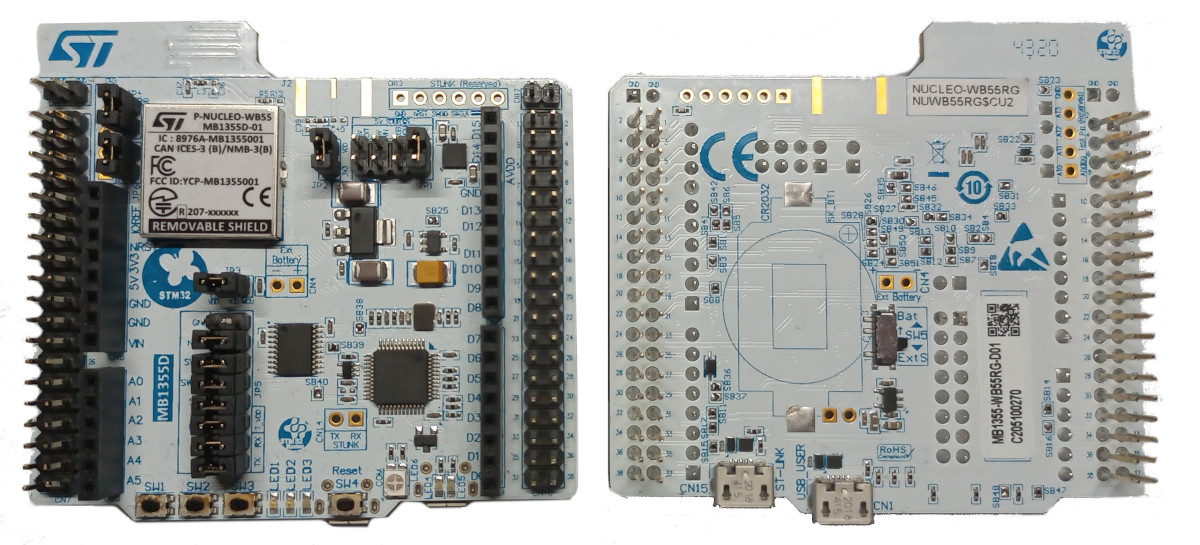
\includegraphics[width=0.618\linewidth]{nucleo_wb55.jpg}
	\caption{Zestaw uruchomieniowy P-NUCLEO-WB55. Źródło: \cite{noauthor_p-nucleo-wb55_nodate}}
	\label{rys:nucleo_wb55}
\end{figure}


\subsubsection{X-NUCLEO-LPM01A}
\begin{figure}[!htb]
	\centering 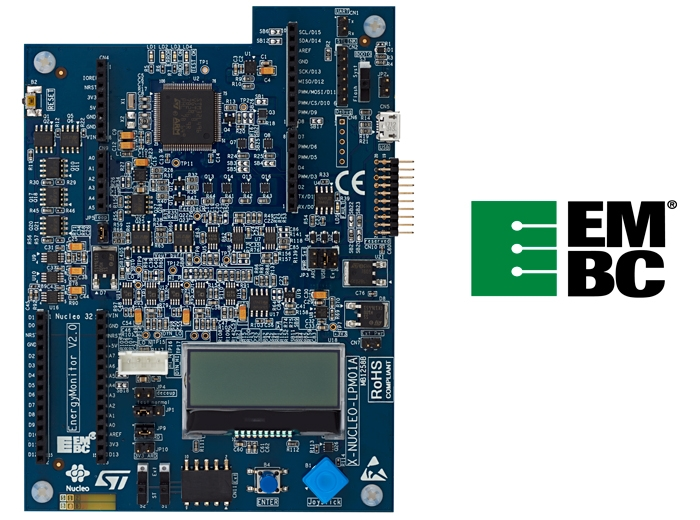
\includegraphics[width=0.618\linewidth]{st_power_measurement_unit.jpg}
	\caption{Zestaw pomiarowy X-NUCLEO-LPM01A. Źródło: \cite{noauthor_x-nucleo-lpm01a_nodate}}
	\label{rys:nucleo_lpm01a}
\end{figure}

\subsubsection{Narzędzia i firmware firmy ST}
Firma ST wraz z zestawem uruchomieniowym udostępnia pełne zintegrowane środowisko
programistyczne oraz niezbędne biblioteki i certyfikowany firmware:

\begin{itemize}
\item \textbf{STM32CubeIDE} \cite{noauthor_stm32cubeide_2022} - multiplatformowe zintegrowane środowisko programistyczne
dostarczane przez ST bazujące na otwartoźródłowym środowisko \textit{Eclipse}\footnote{https://www.eclipse.org/ide/}.
\item \textbf{STM32CubeProgrammer} \cite{noauthor_stm32cubeprog_2022} - narzędzie umożliwiające wykonywanie operacji
odczytu, zapisu i weryfikacji skompilowanego oprogramowania produktów STM32. 
\item \textbf{STM32CubeMonitor-Power} \cite{noauthor_stm32cubemonpwr_2022} - oprogramowanie służące akwizycji danych
o zużyciu energii m.in. w zestawie X-NUCLEO-LPM01A Rysunek: \ref{rys:nucleo_lpm01a}.
\item \textbf{Firmware STM32CubeWB} \cite{noauthor_stm32cubewb_2022} - zestaw bibliotek, narzędzi oraz przykładów
przeznaczonych dla mikrokontrolerów rodziny STM32WB. W skład tego repozytorium wchodzą zależności takie jak:
skompilowany, zamknięty firmware ko-processora dla różnych stosów połączeń bezprzewodowych; przykłady programów
wykorzystujące biblioteki HAL jak i również bezpośrednio rejestry; przykłady BLE; przykłady BLE Mesh.
\end{itemize}
%%%%%%%%%%%%%%%%%%%%%%%%%%%%%%%%%%%%%%%%%%%%%%%%%%%%%%%%%%%%%%%%%%%%%%%%%%%%%%%%
%% SUBSECTION: Zestawy firmy ST: P-NUCLEO-WB55 i X-NUCLEO-LPM01A
%%%%%%%%%%%%%%%%%%%%%%%%%%%%%%%%%%%%%%%%%%%%%%%%%%%%%%%%%%%%%%%%%%%%%%%%%%%%%%%%
\subsection{Zasilanie i obudowy}

\begin{figure}[!htb]
	\centering 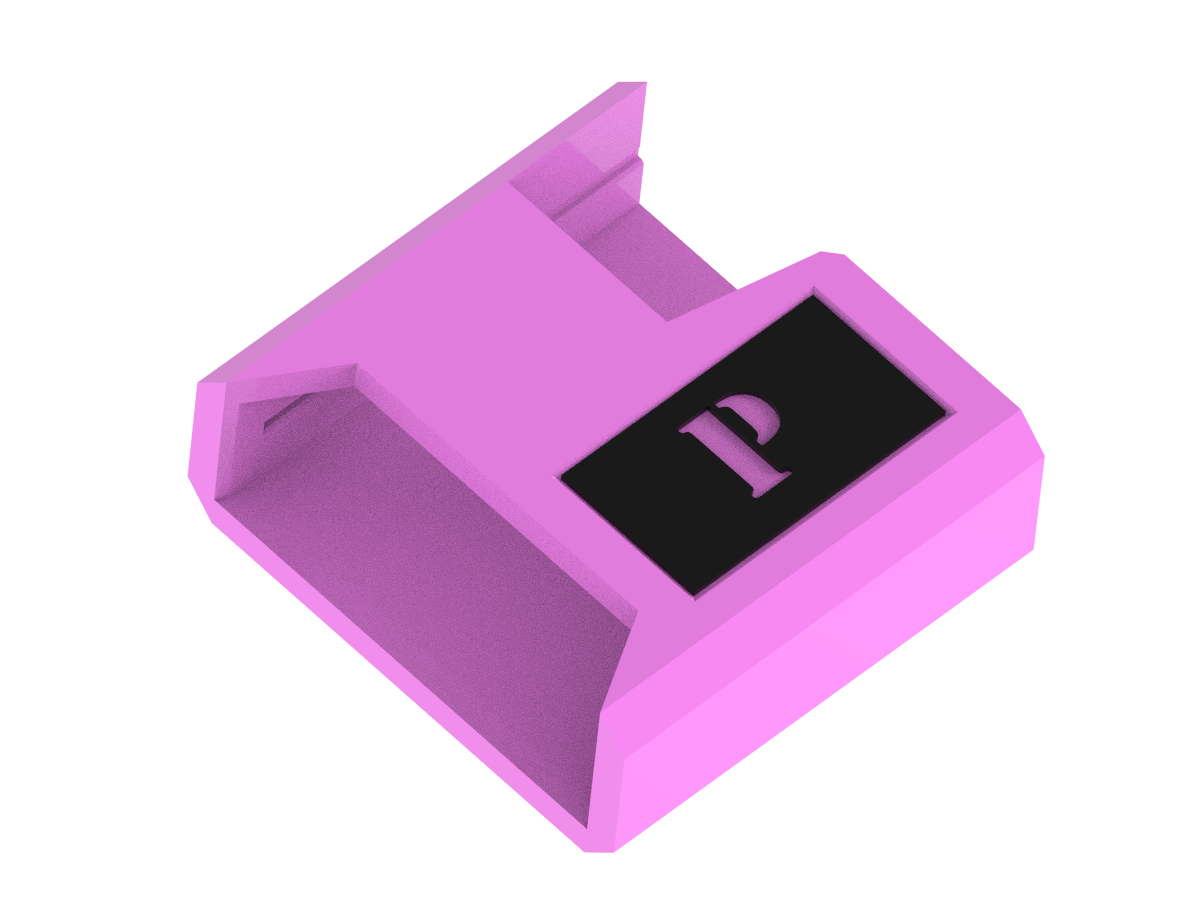
\includegraphics[width=0.618\linewidth]{stm_case_render.png}
	\caption{Obudowa zestawu uruchomieniowego Nucleo wykonana w technologii druku 3D - model}
	\label{rys:obudowa_model3d}
\end{figure}

%%%%%%%%%%%%%%%%%%%%%%%%%%%%%%%%%%%%%%%%%%%%%%%%%%%%%%%%%%%%%%%%%%%%%%%%%%%%%%%%
%% SUBSECTION: Oprogramowanie mikrokontrolera
%%%%%%%%%%%%%%%%%%%%%%%%%%%%%%%%%%%%%%%%%%%%%%%%%%%%%%%%%%%%%%%%%%%%%%%%%%%%%%%%
\subsection{Oprogramowanie mikrokontrolera}

%%%%%%%%%%%%%%%%%%%%%%%%%%%%%%%%%%%%%%%%%%%%%%%%%%%%%%%%%%%%%%%%%%%%%%%%%%%%%%%%
%% SUBSECTION: Oprogramowanie PC
%%%%%%%%%%%%%%%%%%%%%%%%%%%%%%%%%%%%%%%%%%%%%%%%%%%%%%%%%%%%%%%%%%%%%%%%%%%%%%%%
\subsection{Oprogramowanie PC}


%%!!!!!!!!!!!!!!!!!!!!!!!!!!!!!!!!!!!!!!!!!!!!!!!!!!!!!!!!!!!!!!!!!!!!!!!!!!!!!!
%%%%%%%%%%%%%%%%%%%%%%%%%%%%%%%%%%%%%%%%%%%%%%%%%%%%%%%%%%%%%%%%%%%%%%%%%%%%%%%%
%% SECTION: Zużycie energii
%%%%%%%%%%%%%%%%%%%%%%%%%%%%%%%%%%%%%%%%%%%%%%%%%%%%%%%%%%%%%%%%%%%%%%%%%%%%%%%%
%%!!!!!!!!!!!!!!!!!!!!!!!!!!!!!!!!!!!!!!!!!!!!!!!!!!!!!!!!!!!!!!!!!!!!!!!!!!!!!!
\section{Zużycie energii}

%%%%%%%%%%%%%%%%%%%%%%%%%%%%%%%%%%%%%%%%%%%%%%%%%%%%%%%%%%%%%%%%%%%%%%%%%%%%%%%%
%% SUBSECTION: Metodologia badania
%%%%%%%%%%%%%%%%%%%%%%%%%%%%%%%%%%%%%%%%%%%%%%%%%%%%%%%%%%%%%%%%%%%%%%%%%%%%%%%%
\subsection{Metodologia badania}

%%%%%%%%%%%%%%%%%%%%%%%%%%%%%%%%%%%%%%%%%%%%%%%%%%%%%%%%%%%%%%%%%%%%%%%%%%%%%%%%
%% SUBSECTION: BT Low Energy - Usługa Heart Rate
%%%%%%%%%%%%%%%%%%%%%%%%%%%%%%%%%%%%%%%%%%%%%%%%%%%%%%%%%%%%%%%%%%%%%%%%%%%%%%%%
\subsection{BT Low Energy - Usługa Heart Rate}

\begin{figure}[!htb]
	\centering 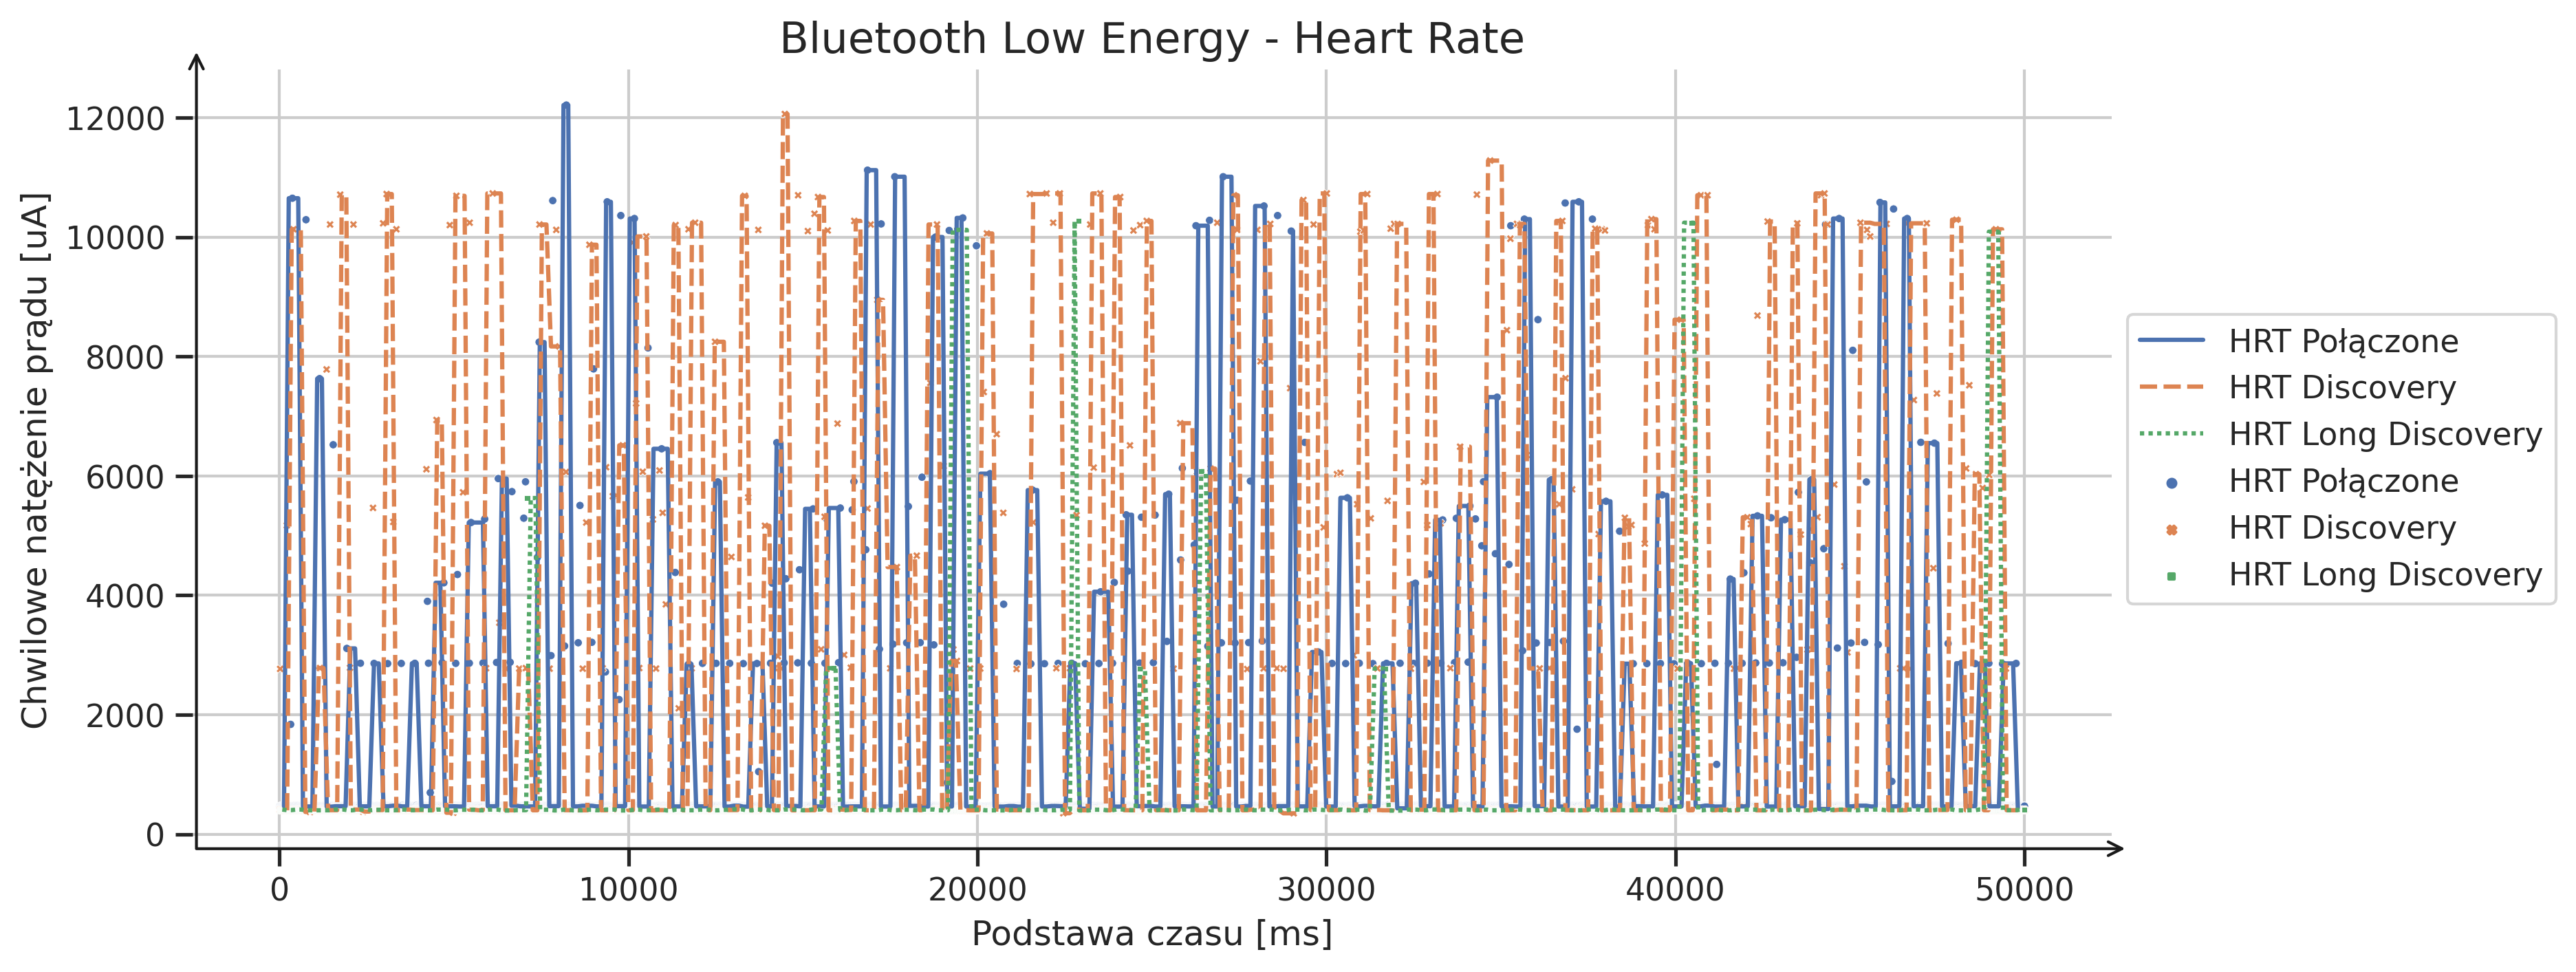
\includegraphics[width=0.99\linewidth]{power_ble_hr_amps.png}
	\caption{Charakterystyka czasowa poboru prądu dla BLE i usługi Heart Rate}
	\label{rys:power_ble_hr_amps}
\end{figure}

\begin{figure}[!htb]
	\centering 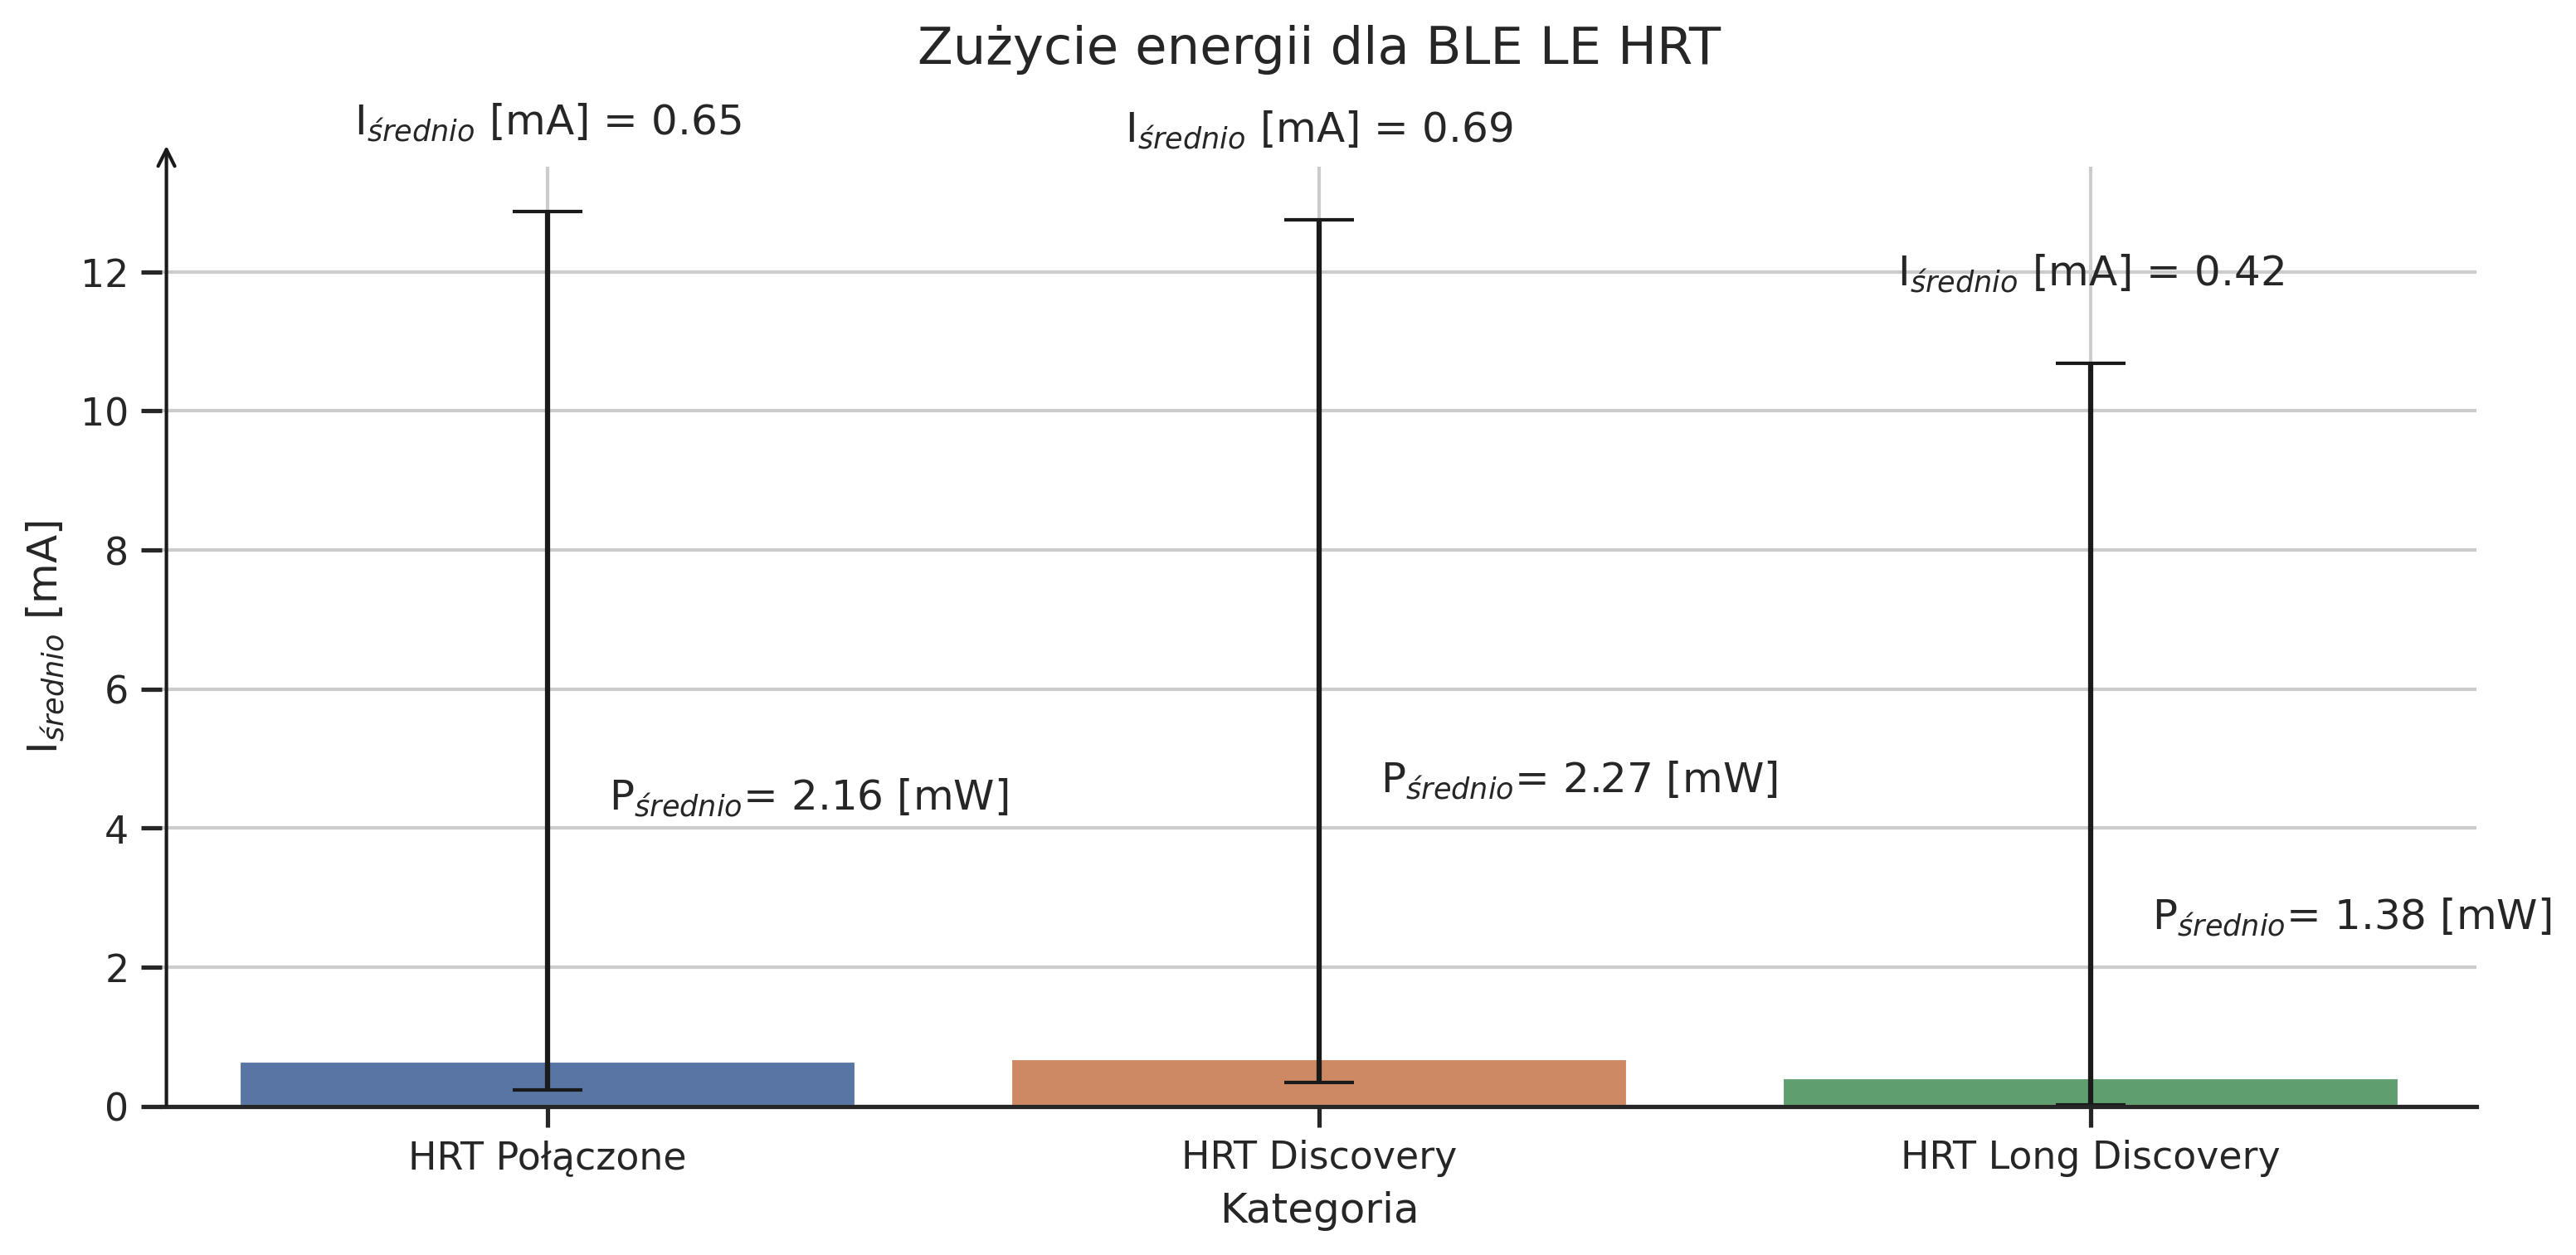
\includegraphics[width=0.99\linewidth]{power_ble_hr_amps_usage_juxtaposition.png}
	\caption{Zestawienie zużycia prądu dla usługi Heart Rate w zależności od trybu działania}
	\label{rys:power_ble_hr_amps_usage_juxtaposition}
\end{figure}

%%%%%%%%%%%%%%%%%%%%%%%%%%%%%%%%%%%%%%%%%%%%%%%%%%%%%%%%%%%%%%%%%%%%%%%%%%%%%%%%
%% SUBSECTION: BLE Mesh - Model Generic OnOff
%%%%%%%%%%%%%%%%%%%%%%%%%%%%%%%%%%%%%%%%%%%%%%%%%%%%%%%%%%%%%%%%%%%%%%%%%%%%%%%%
\subsection{BLE Mesh - Model Generic OnOff}

Pomiary dla BLE Mesh uwzględniające dwa tryby działania: sieć w oczekująca na komunikaty oraz podczas działania aktywnego korzystania z Modelu Generic OnOff.

\begin{figure}[!htb]
	\centering 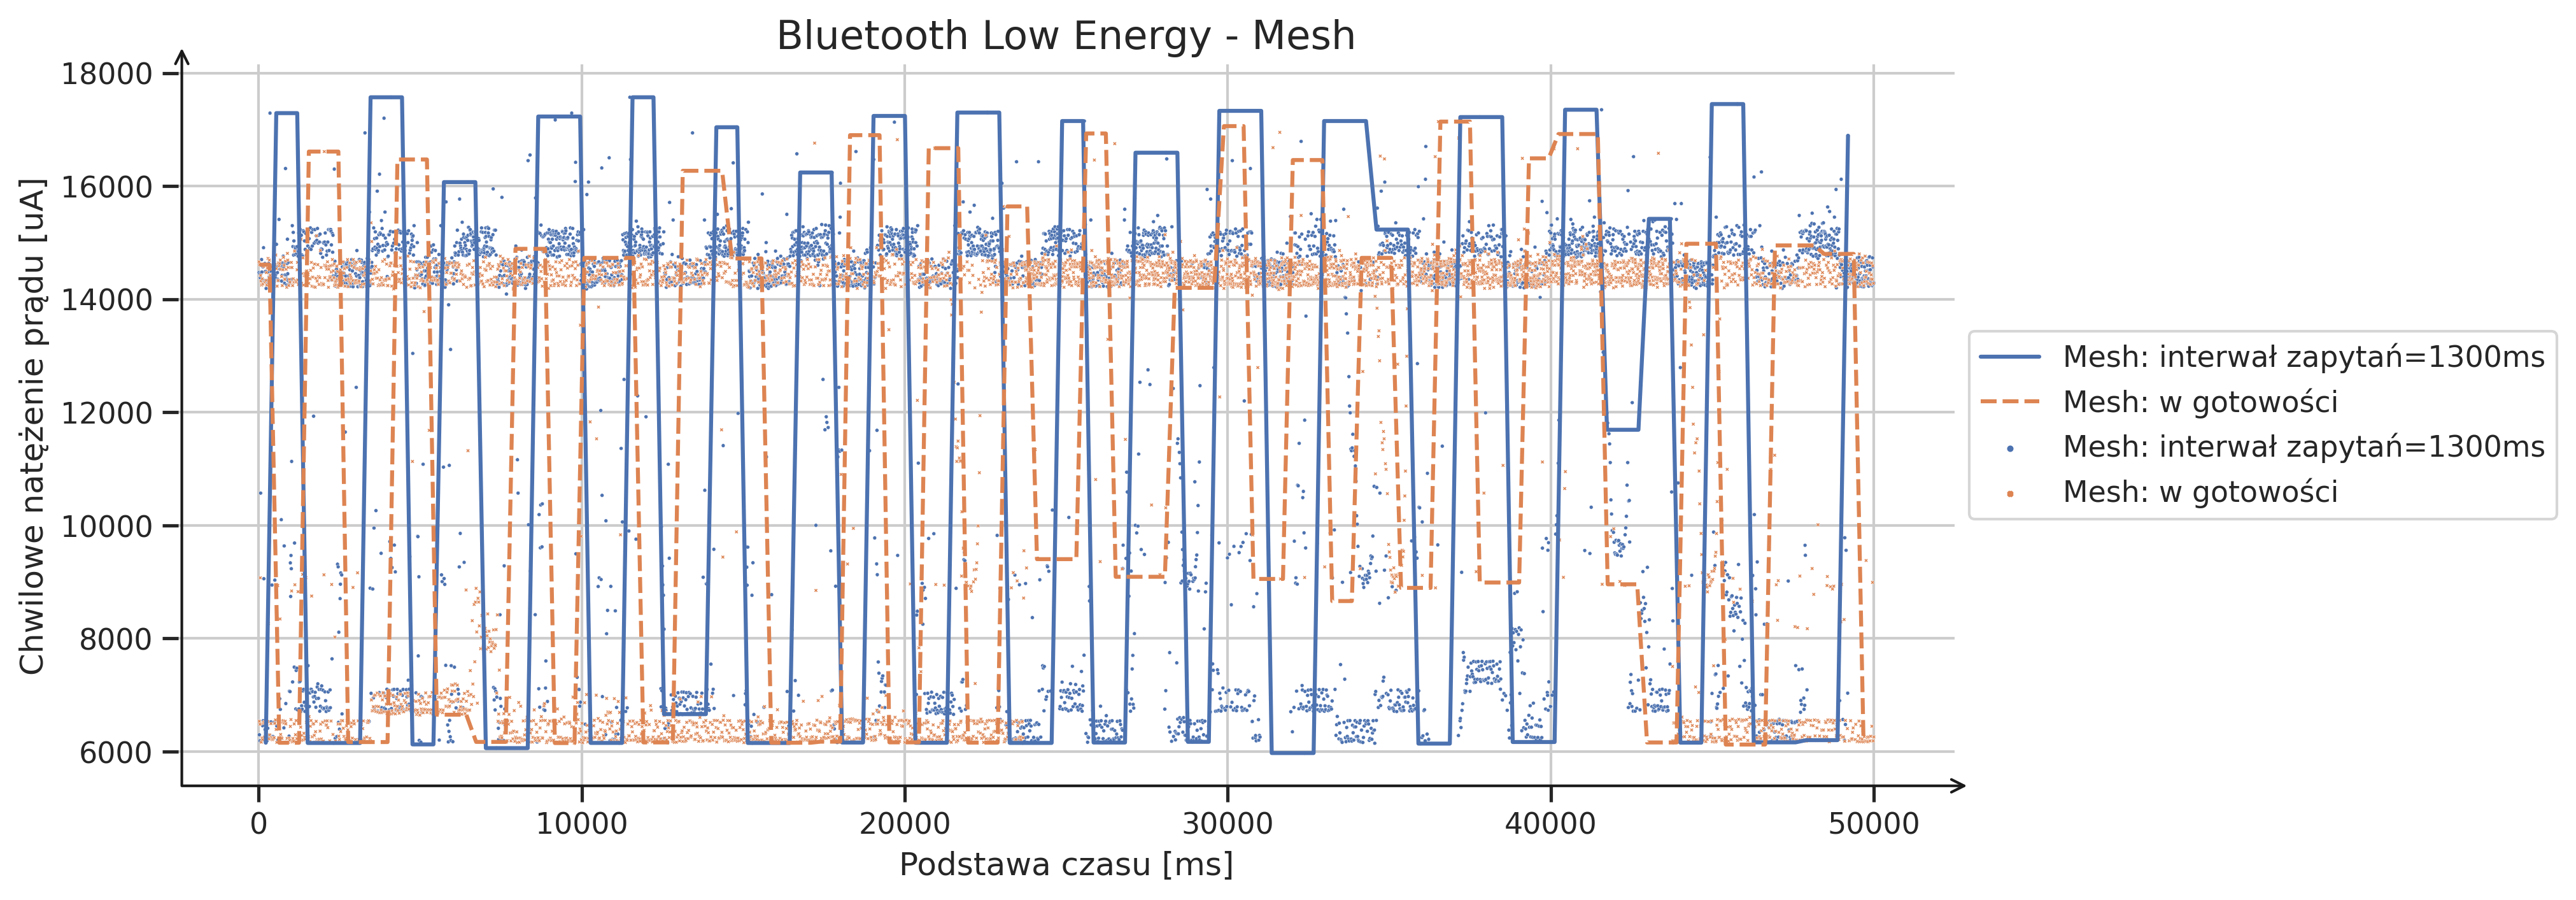
\includegraphics[width=0.99\linewidth]{power_ble_mesh_amps.png} 
	\caption{Charakterystyka czasowa poboru prądu dla BLE Mesh i modelu Generic OnOff}
	\label{rys:power_ble_mesh_amps}
\end{figure}

\begin{figure}[!htb]
	\centering 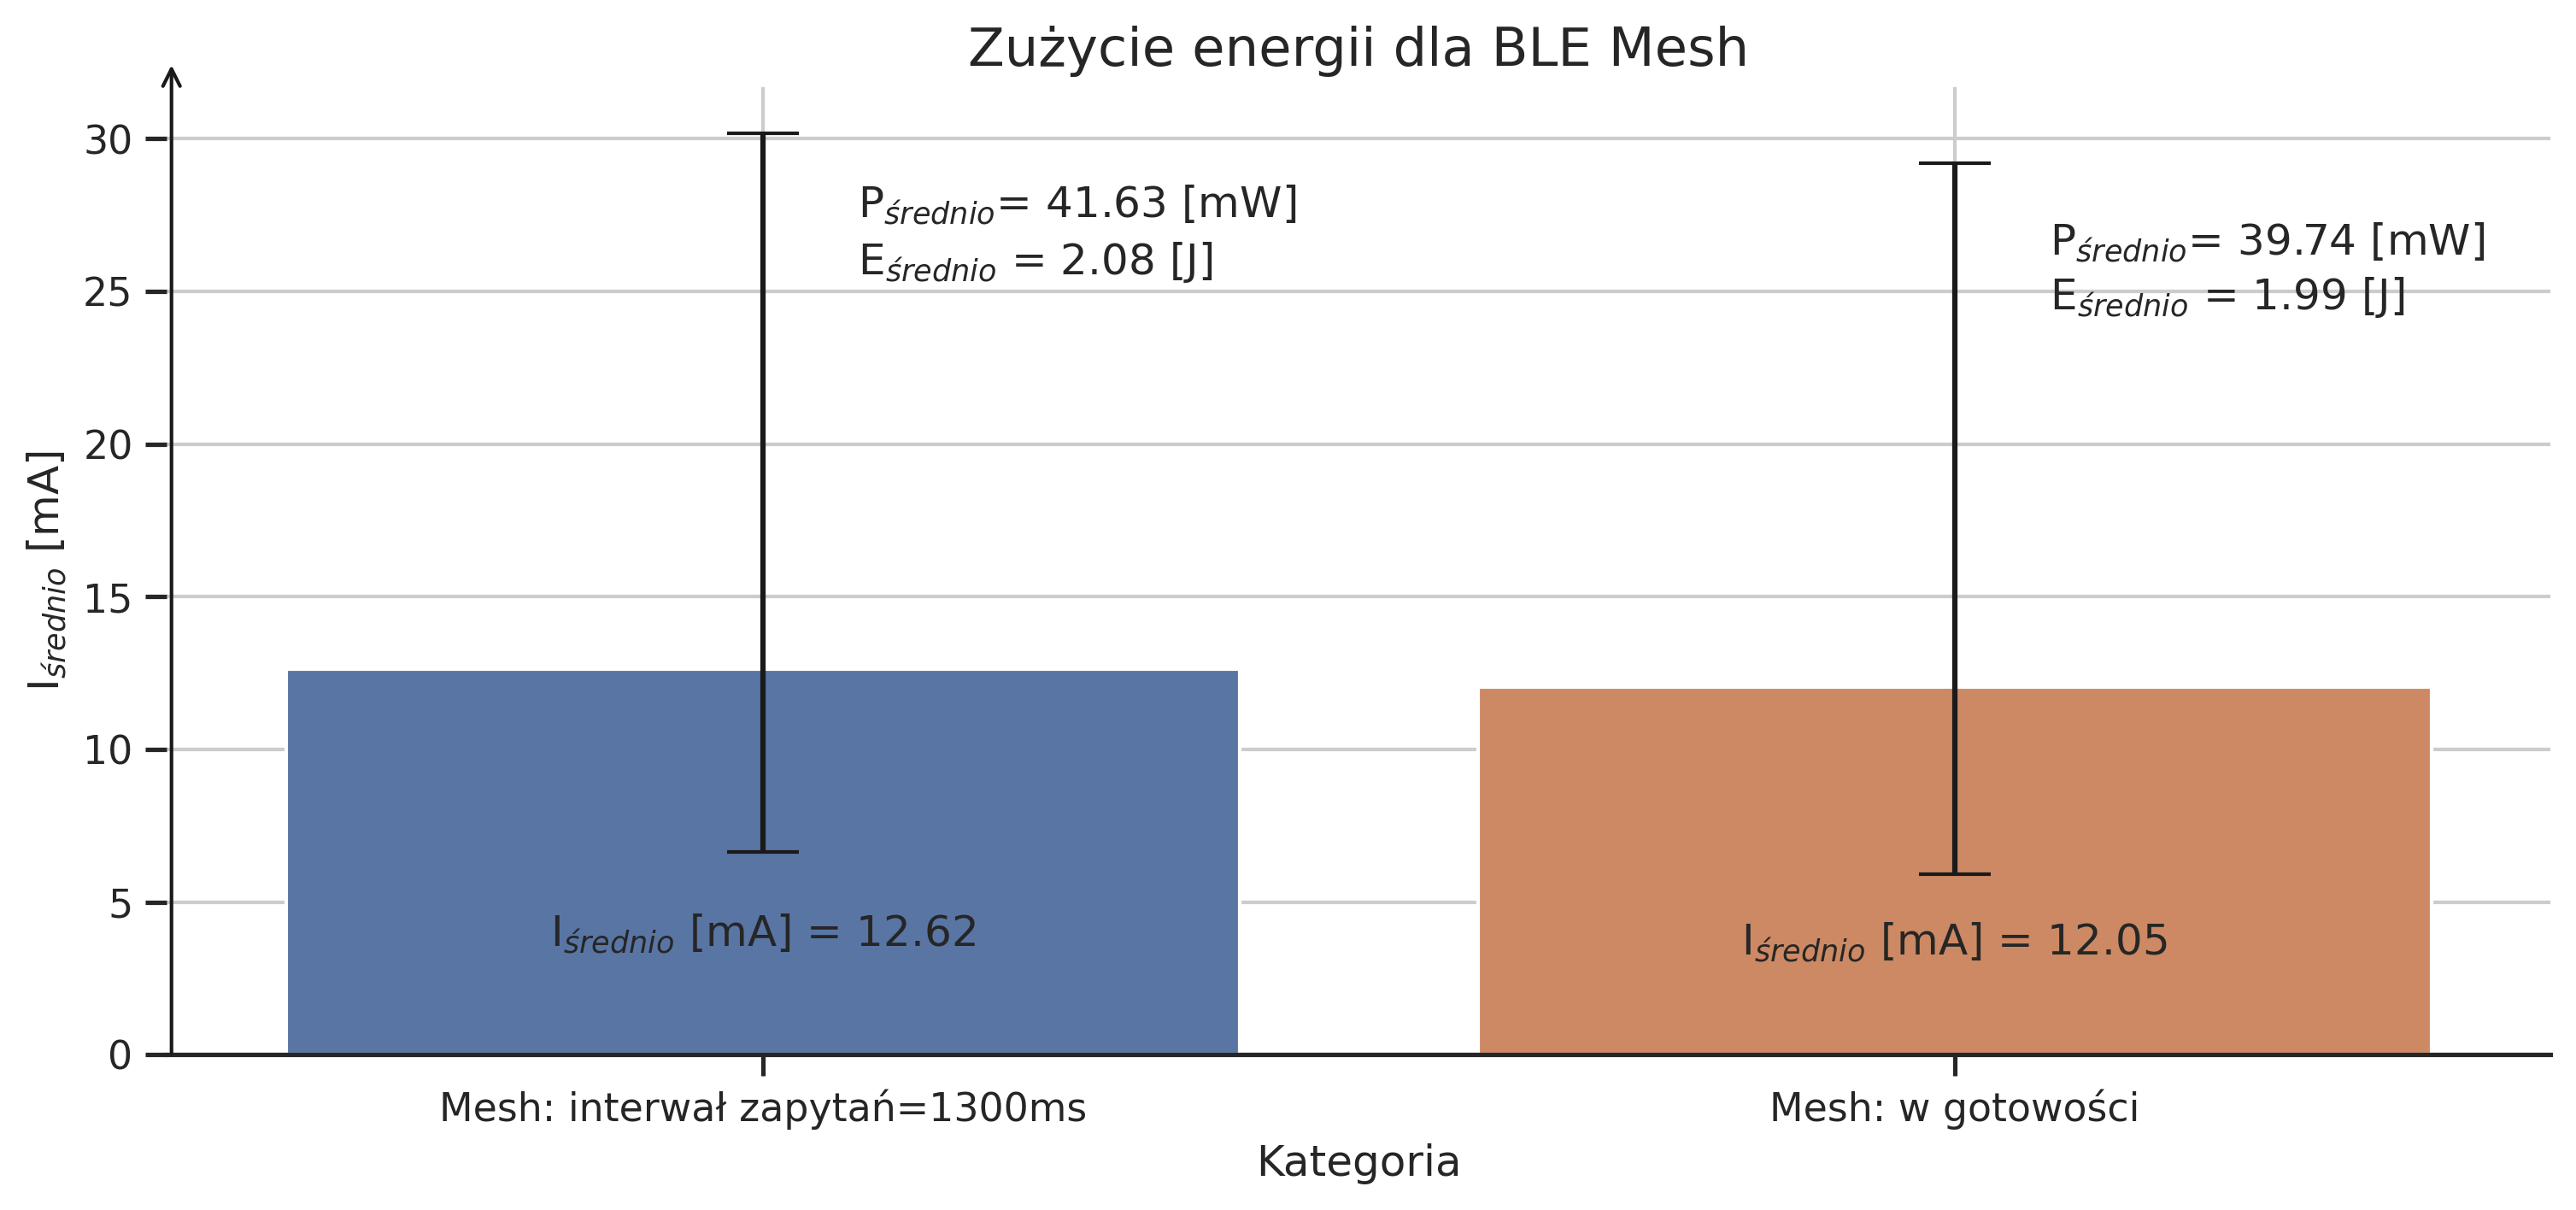
\includegraphics[width=0.99\linewidth]{power_ble_mesh_amps_usage_juxtaposition.png} 
	\caption{Zestawienie zużycia prądu dla BLE Mesh w zależności od trybu działania}
	\label{rys:power_ble_mesh_amps_usage_juxtaposition}
\end{figure}

\begin{figure}[!htb]
	\centering 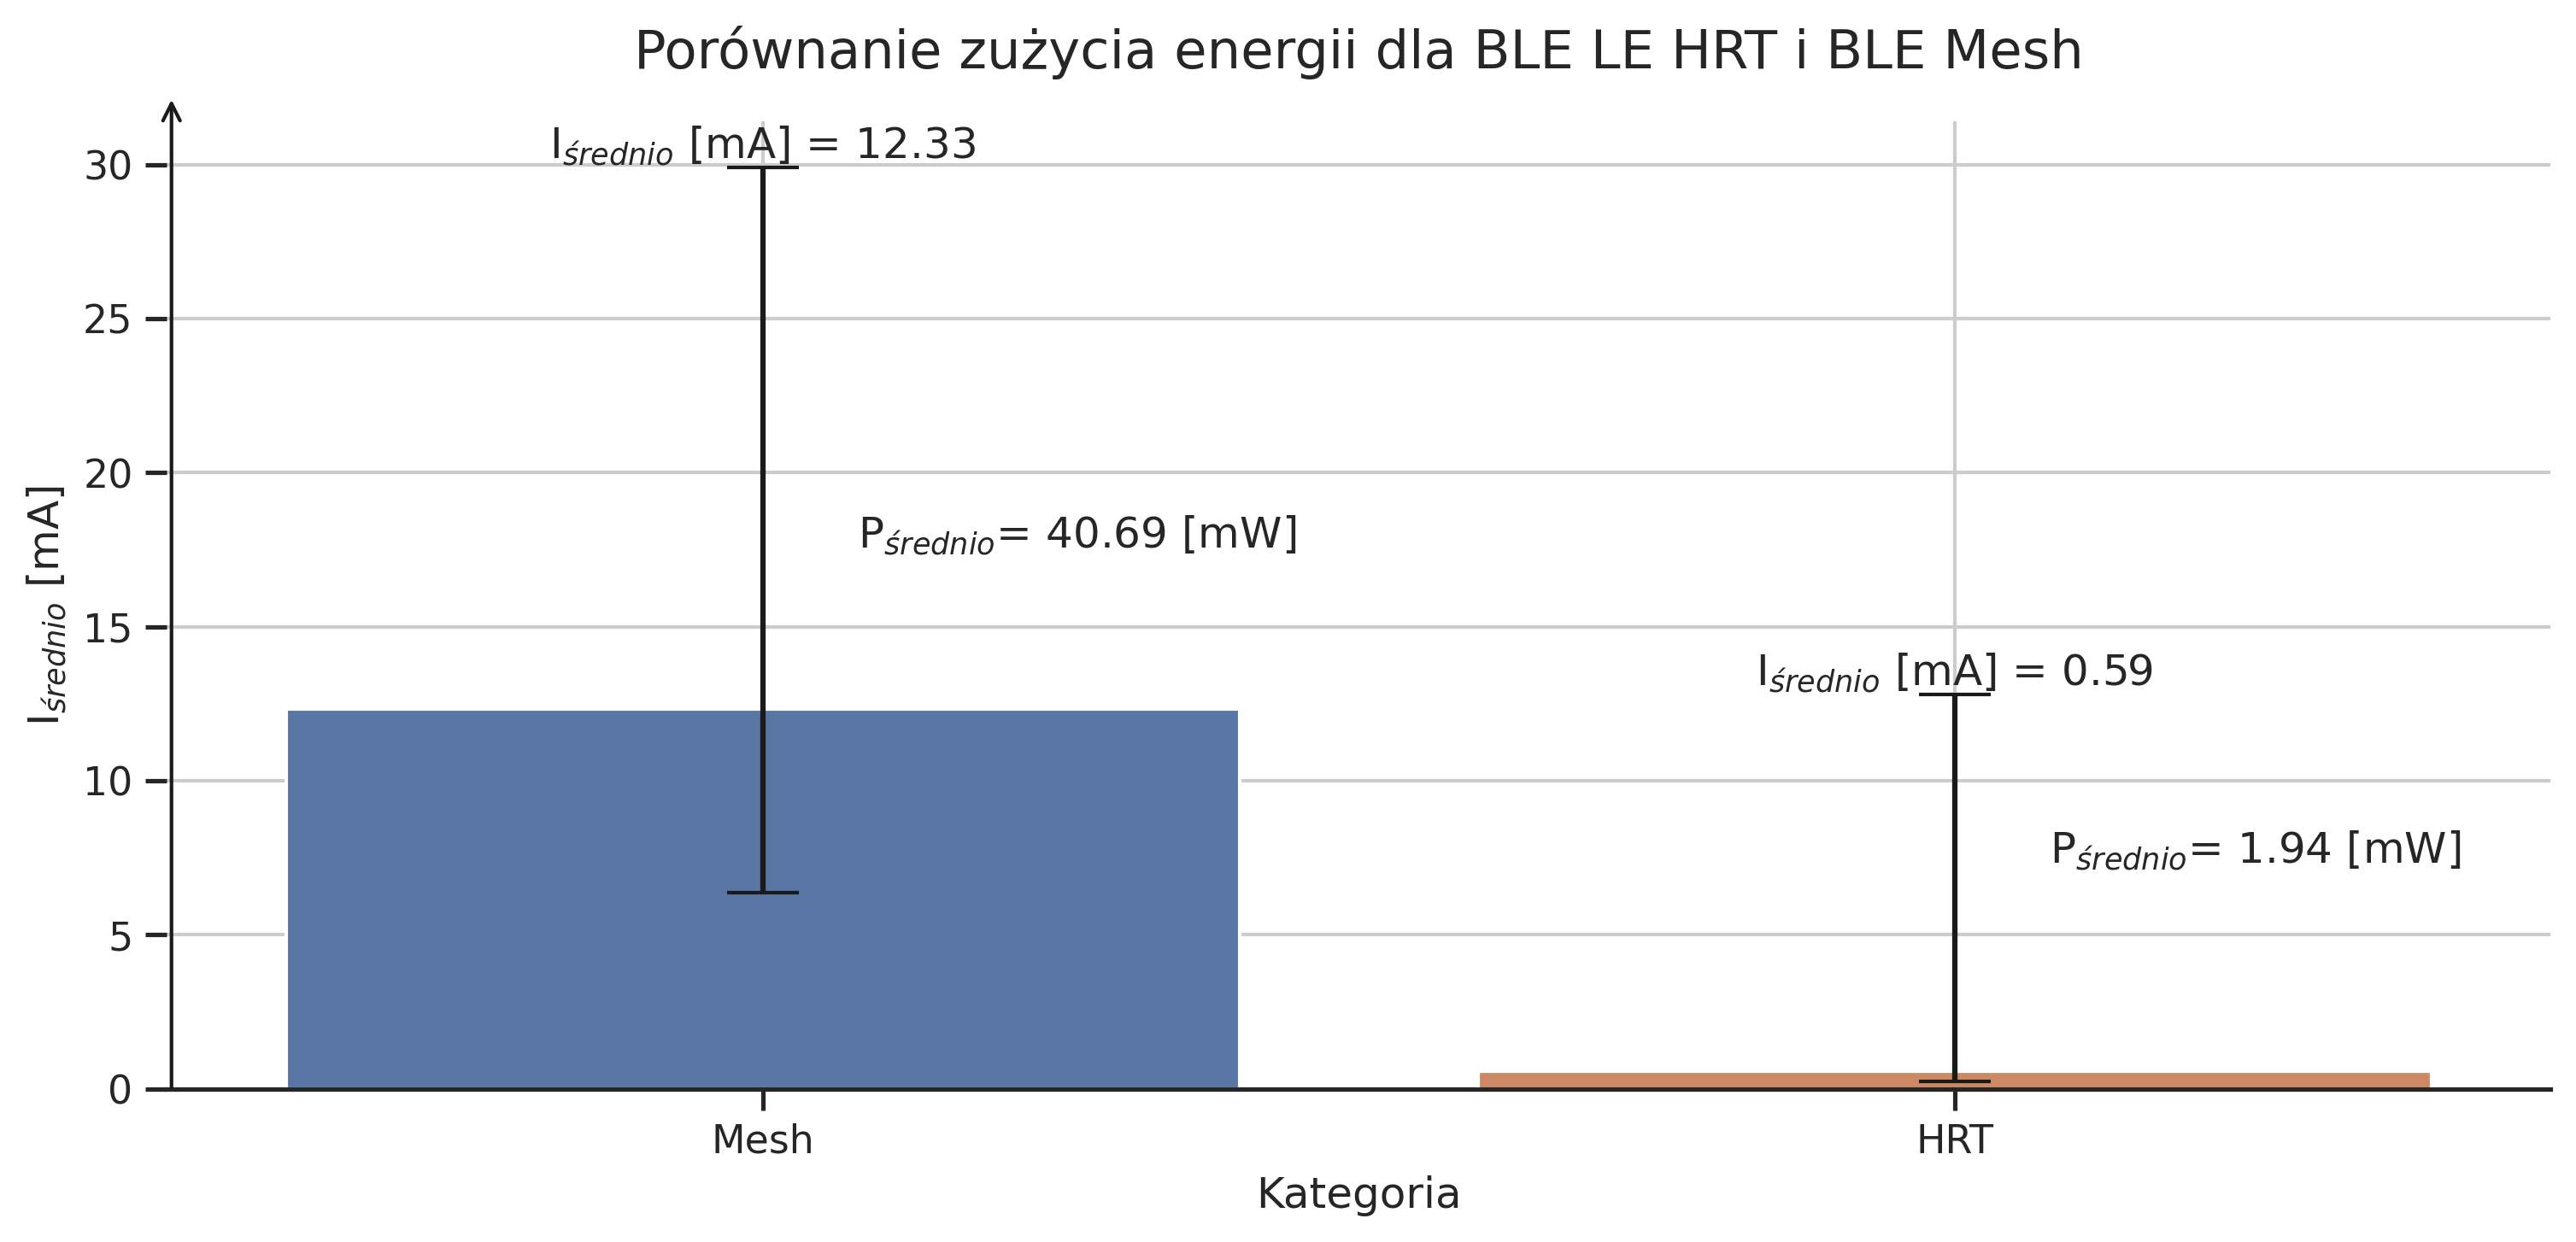
\includegraphics[width=0.99\linewidth]{power_ble_consumption_comparison.png} 
	\caption{Porównanie średniego zużycia energii pomiędzy BT Low Energy HRT i BLE Mesh}
	\label{rys:power_ble_consumption_comparison}
\end{figure}



%%!!!!!!!!!!!!!!!!!!!!!!!!!!!!!!!!!!!!!!!!!!!!!!!!!!!!!!!!!!!!!!!!!!!!!!!!!!!!!!
%%%%%%%%%%%%%%%%%%%%%%%%%%%%%%%%%%%%%%%%%%%%%%%%%%%%%%%%%%%%%%%%%%%%%%%%%%%%%%%%
%% SECTION: Packet Error Rate
%%%%%%%%%%%%%%%%%%%%%%%%%%%%%%%%%%%%%%%%%%%%%%%%%%%%%%%%%%%%%%%%%%%%%%%%%%%%%%%%
%%!!!!!!!!!!!!!!!!!!!!!!!!!!!!!!!!!!!!!!!!!!!!!!!!!!!!!!!!!!!!!!!!!!!!!!!!!!!!!!
\section{Packet Error Rate}

%%%%%%%%%%%%%%%%%%%%%%%%%%%%%%%%%%%%%%%%%%%%%%%%%%%%%%%%%%%%%%%%%%%%%%%%%%%%%%%%
%% SUBSECTION: Zależność PER względem odległości między węzłami
%%%%%%%%%%%%%%%%%%%%%%%%%%%%%%%%%%%%%%%%%%%%%%%%%%%%%%%%%%%%%%%%%%%%%%%%%%%%%%%%
\subsection{Metodologia badania}

\begin{figure}[!htb]
	\centering 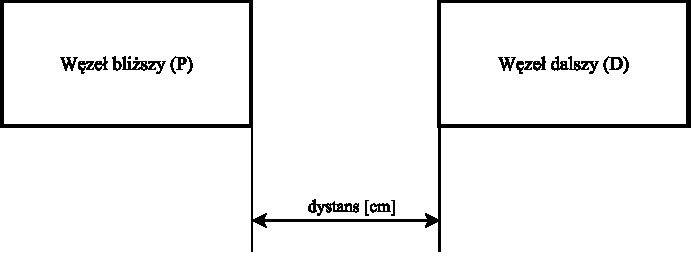
\includegraphics[width=0.618\linewidth]{per_two_nodes.pdf} 
	\caption{Dystans pomiędzy węzłami dla sieci dwóch mikrokontrolerów}
	\label{rys:two_nodes_setup}
\end{figure}

Rysunek ~\ref{rys:two_nodes_setup}

\begin{figure}[!htb]
	\centering 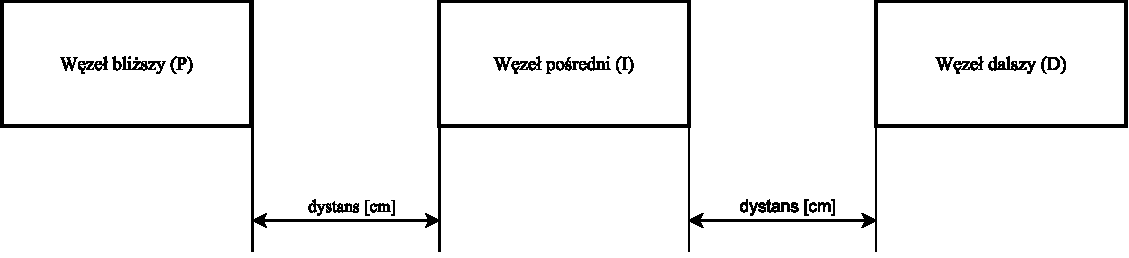
\includegraphics[width=0.99\linewidth]{per_three_nodes.pdf} 
	\caption{Dystans pomiędzy węzłami dla sieci trzech mikrokontrolerów}
	\label{rys:three_nodes_setup}
\end{figure}

%%%%%%%%%%%%%%%%%%%%%%%%%%%%%%%%%%%%%%%%%%%%%%%%%%%%%%%%%%%%%%%%%%%%%%%%%%%%%%%%
%% SUBSECTION: Zależność PER względem częstości zapytań
%%%%%%%%%%%%%%%%%%%%%%%%%%%%%%%%%%%%%%%%%%%%%%%%%%%%%%%%%%%%%%%%%%%%%%%%%%%%%%%%
\subsection{Zależność PER względem częstości zapytań}

\begin{figure}[!htb]
	\centering 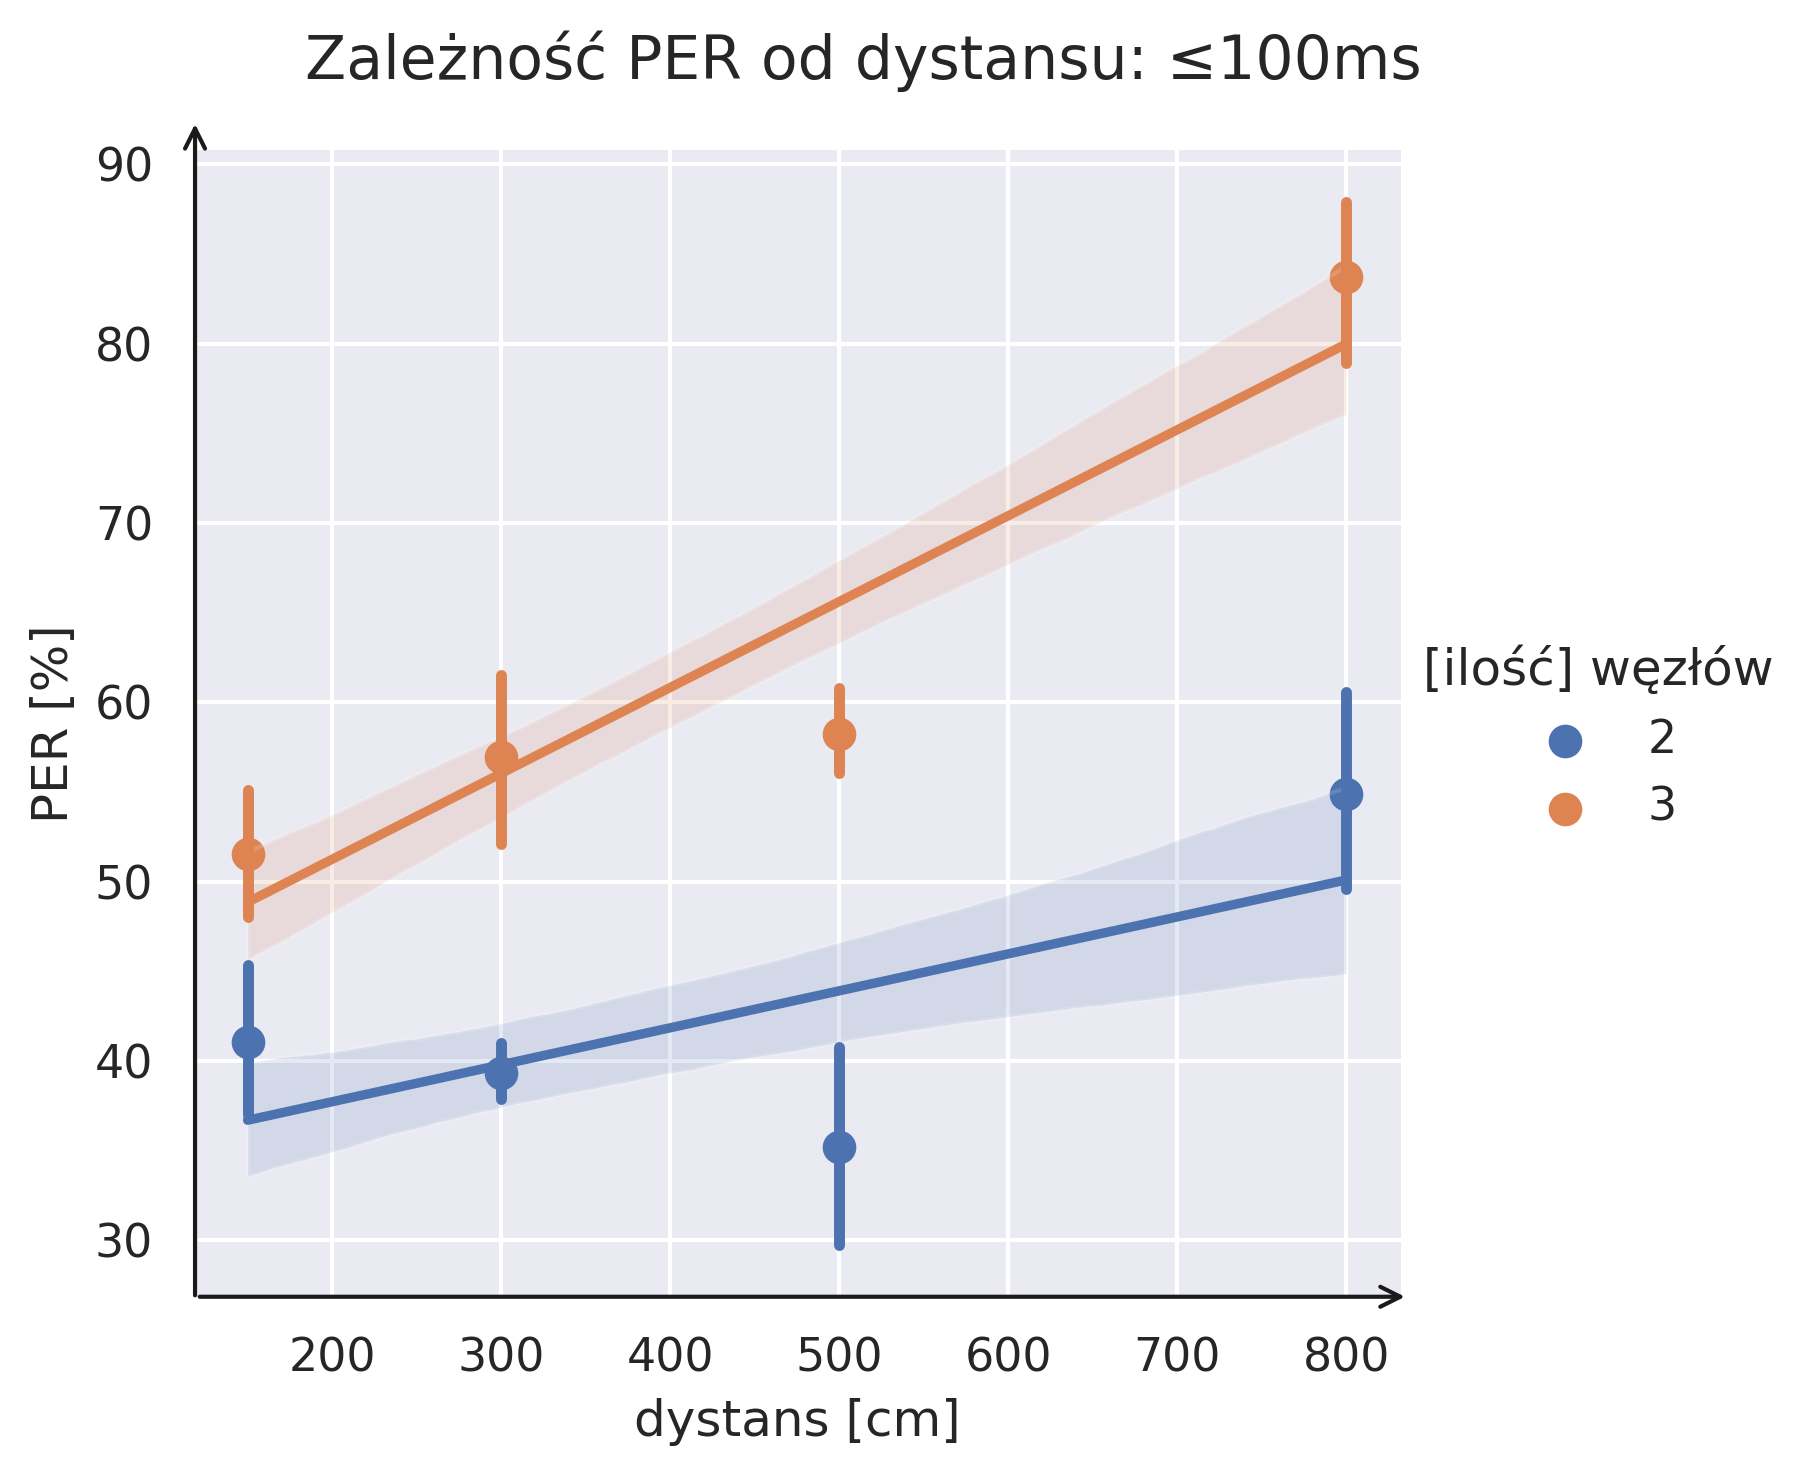
\includegraphics[width=0.618\linewidth]{per_to_distance_under_100ms.png}
	\caption{Zależność PER od dystansu dla zapytań o częstości $\leqslant$ 100ms dla różnej liczby węzłów}
	\label{rys:per_to_distance_under_100ms}
\end{figure}

\begin{figure}[!htb]
	\centering 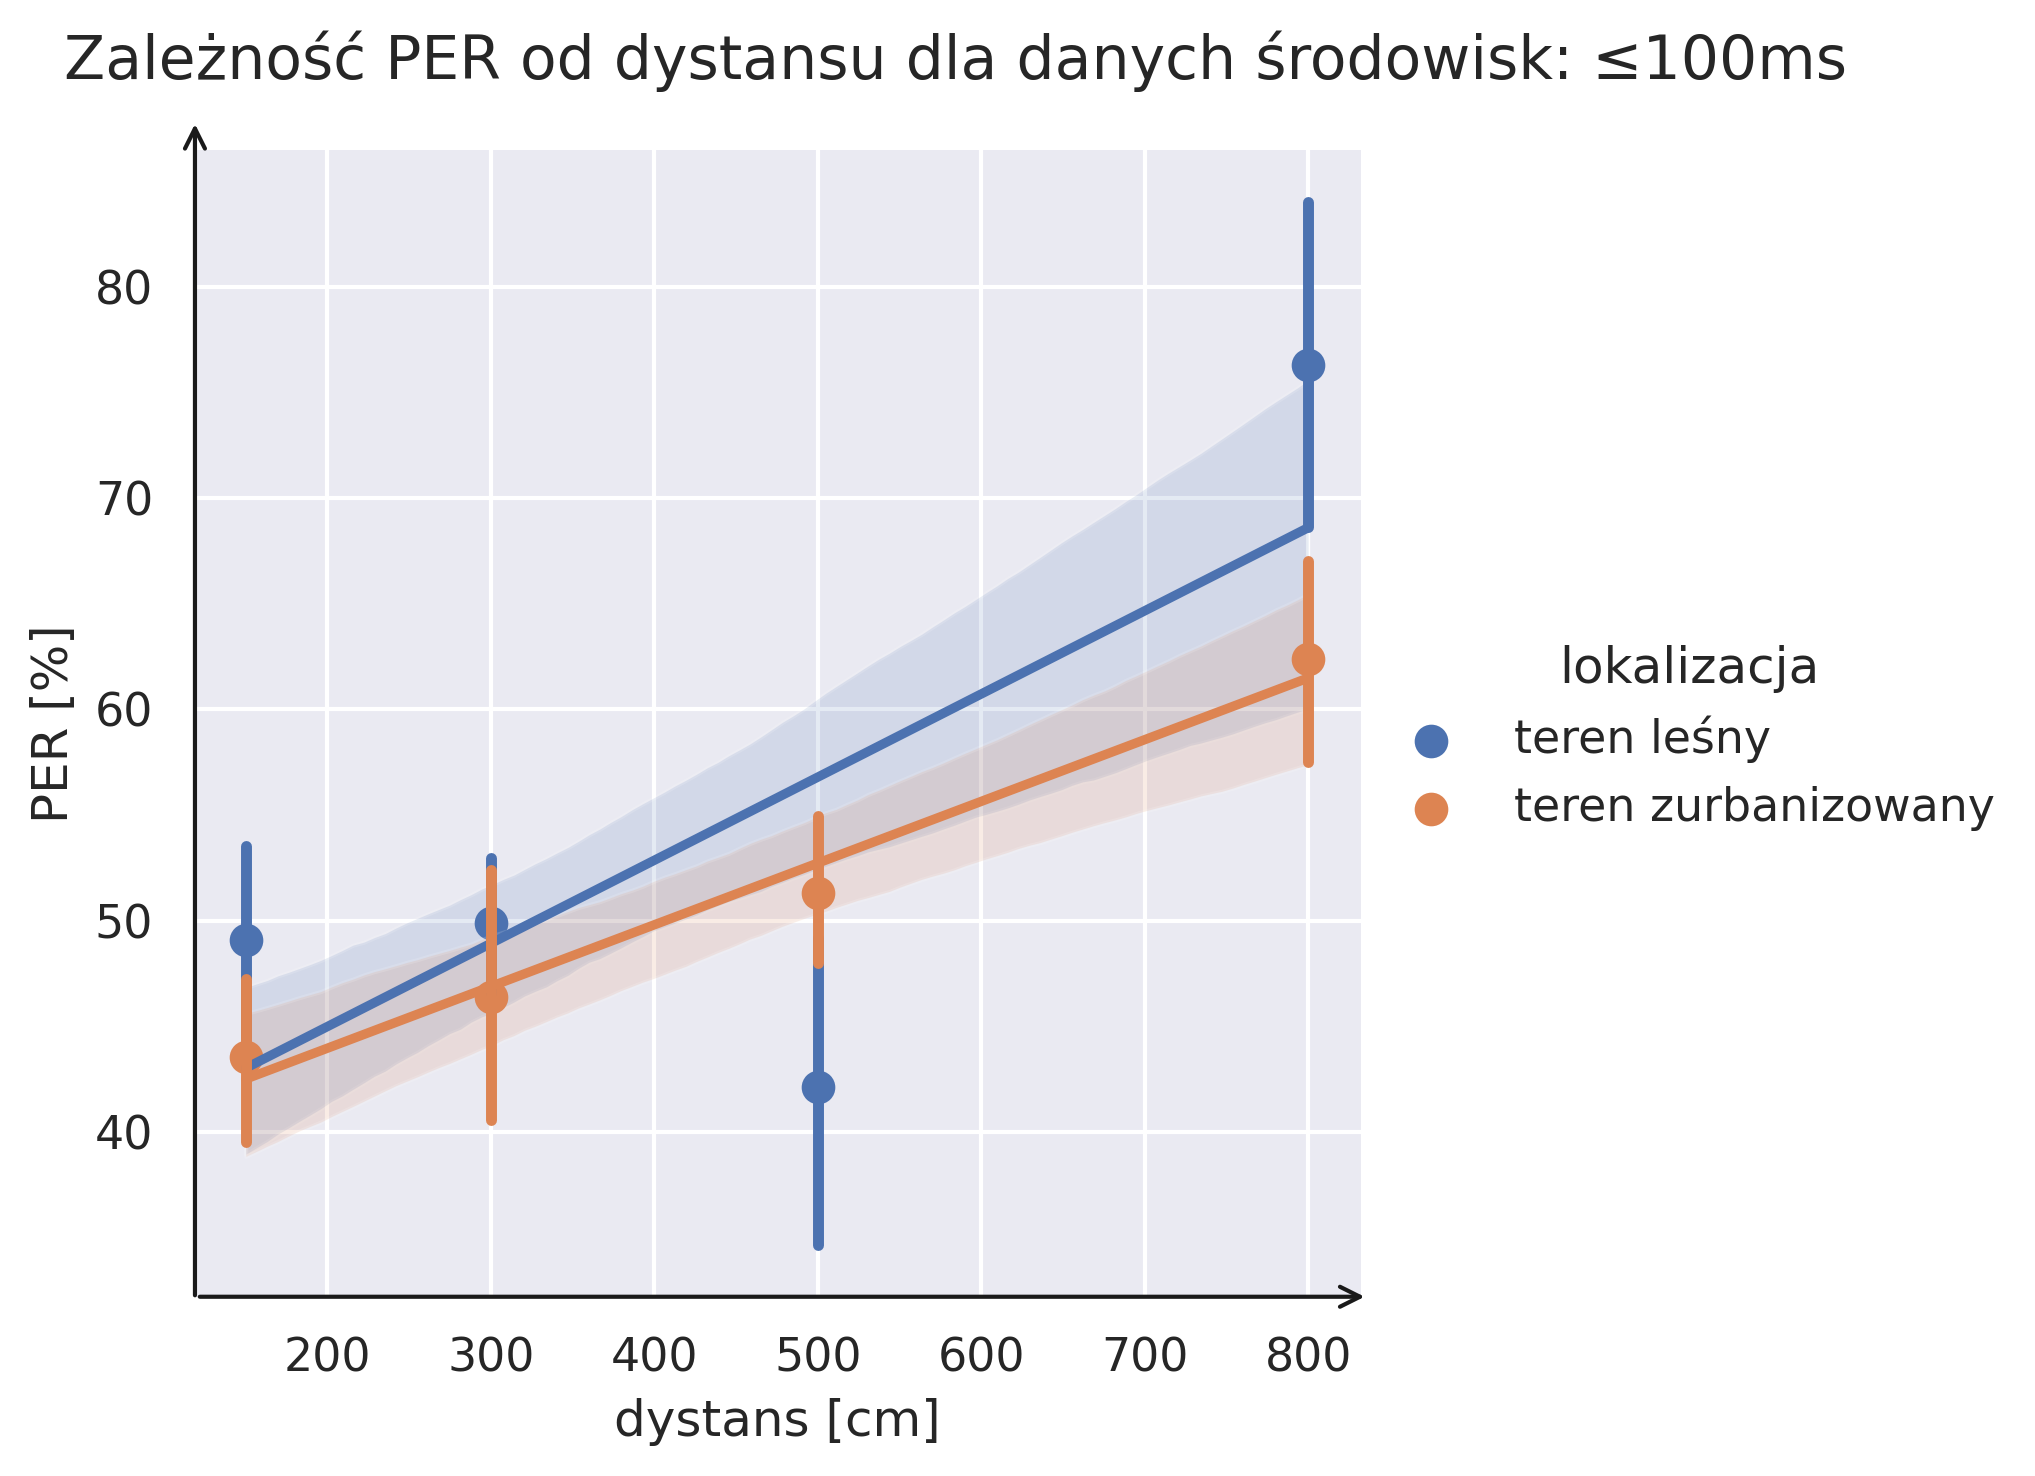
\includegraphics[width=0.618\linewidth]{per_to_distance_under_100ms_different_envs.png} 
	\caption{Zależność PER od dystansu dla zapytań o częstości $\leqslant$ 100ms w wybranych środowiskach bez rozróżnienia na liczbę węzłów}
	\label{rys:per_to_distance_under_100ms_different_envs}
\end{figure}

\begin{figure}[!htb]
	\centering 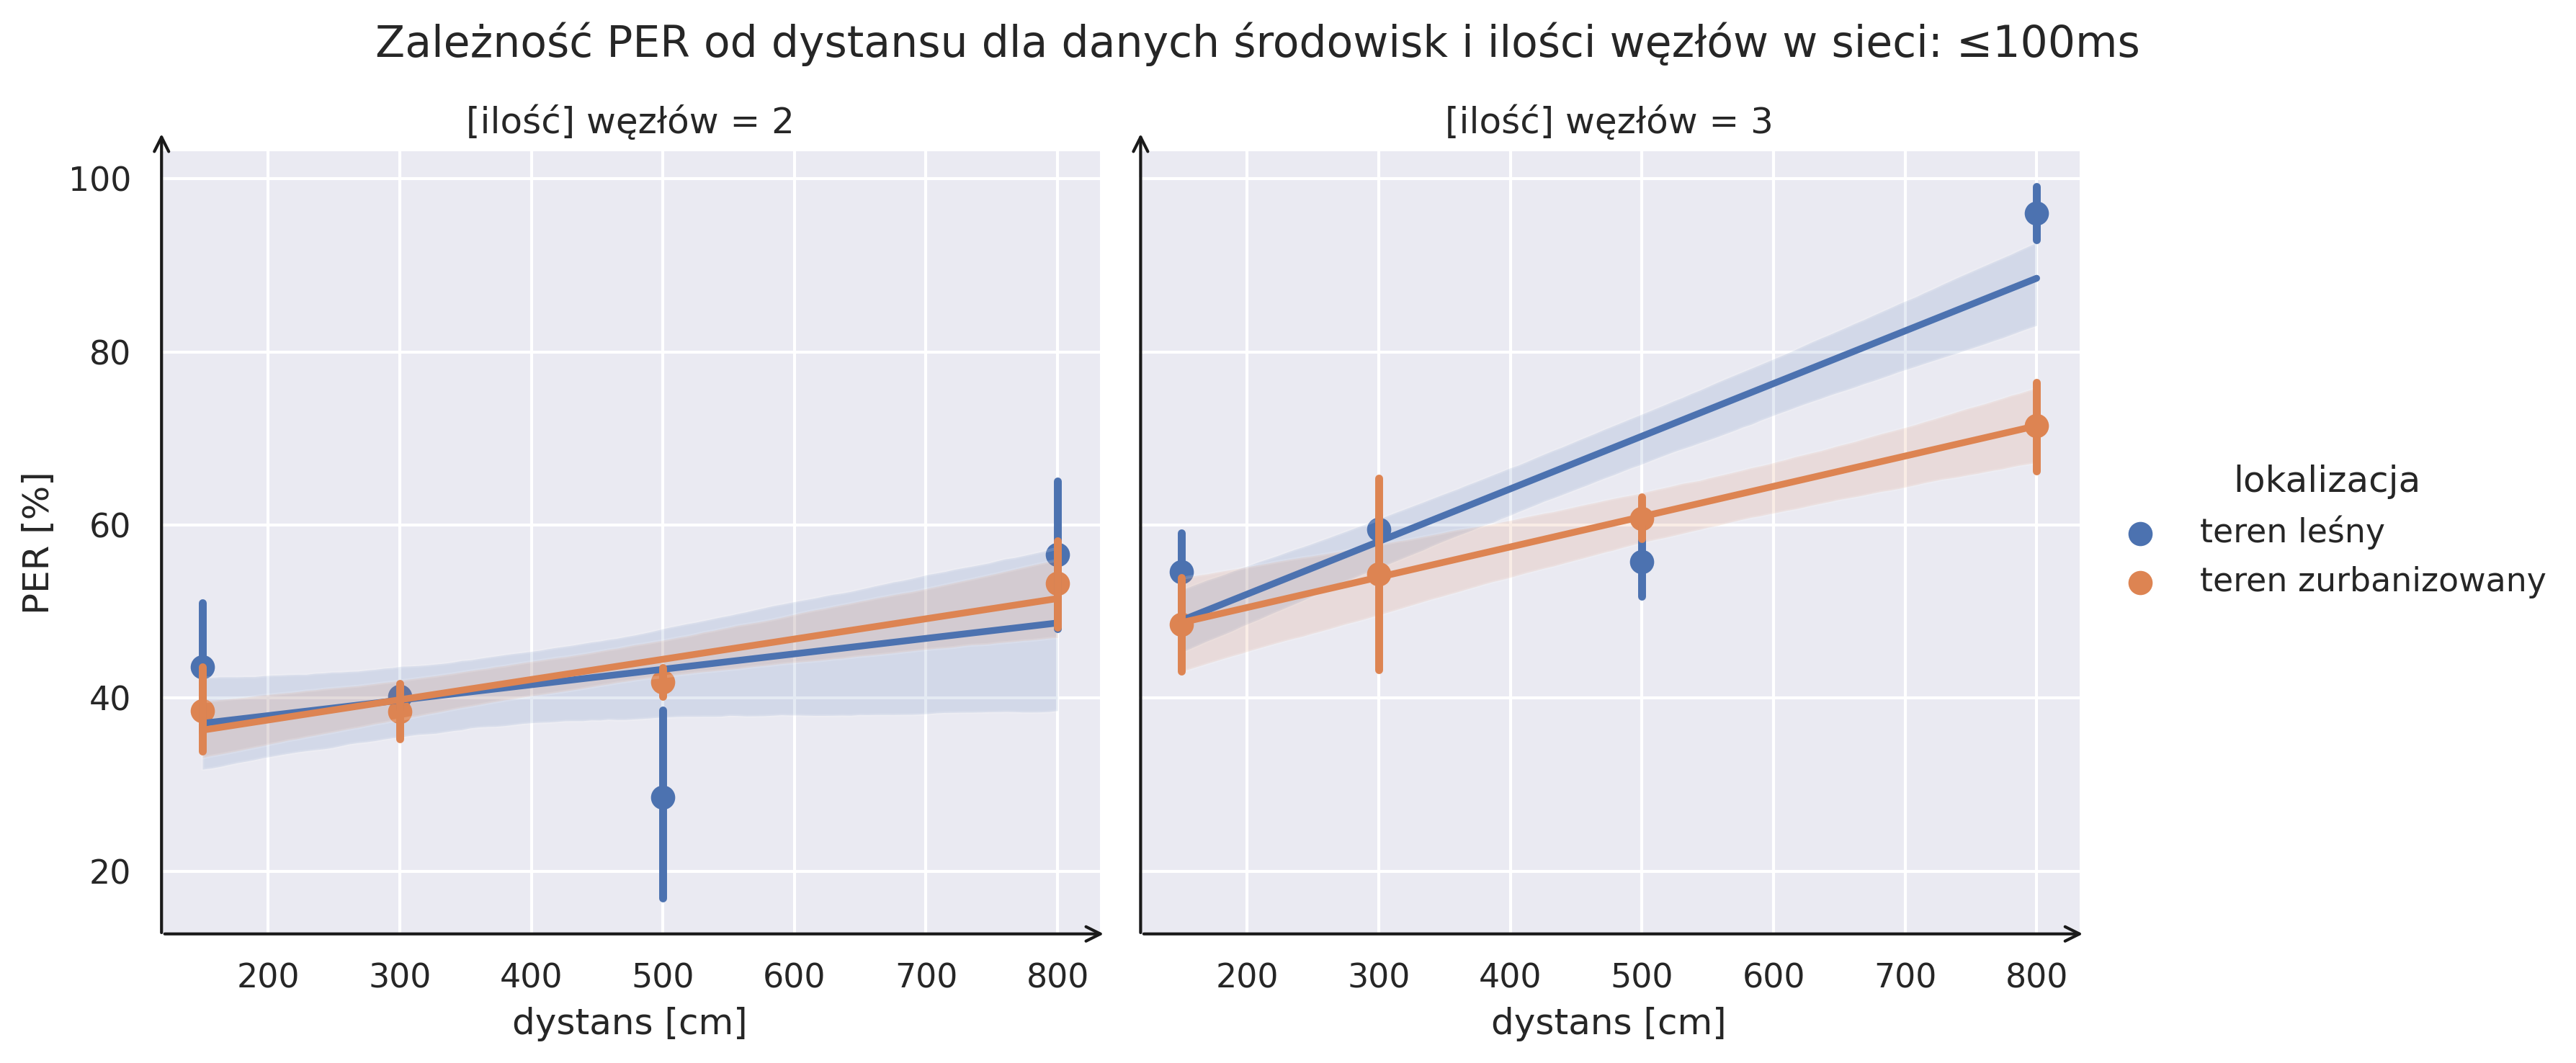
\includegraphics[width=0.99\linewidth]{per_to_distance_under_100ms_different_envs_and_nodes.png}
	\caption{Zależność PER od dystansu dla zapytań o częstości $\leqslant$ 100ms w wybranych środowiskach i liczbę badanych węzłów}
	\label{rys:per_to_distance_under_100ms_different_envs_and_nodes}
\end{figure}

\begin{figure}[!htb]
	\centering 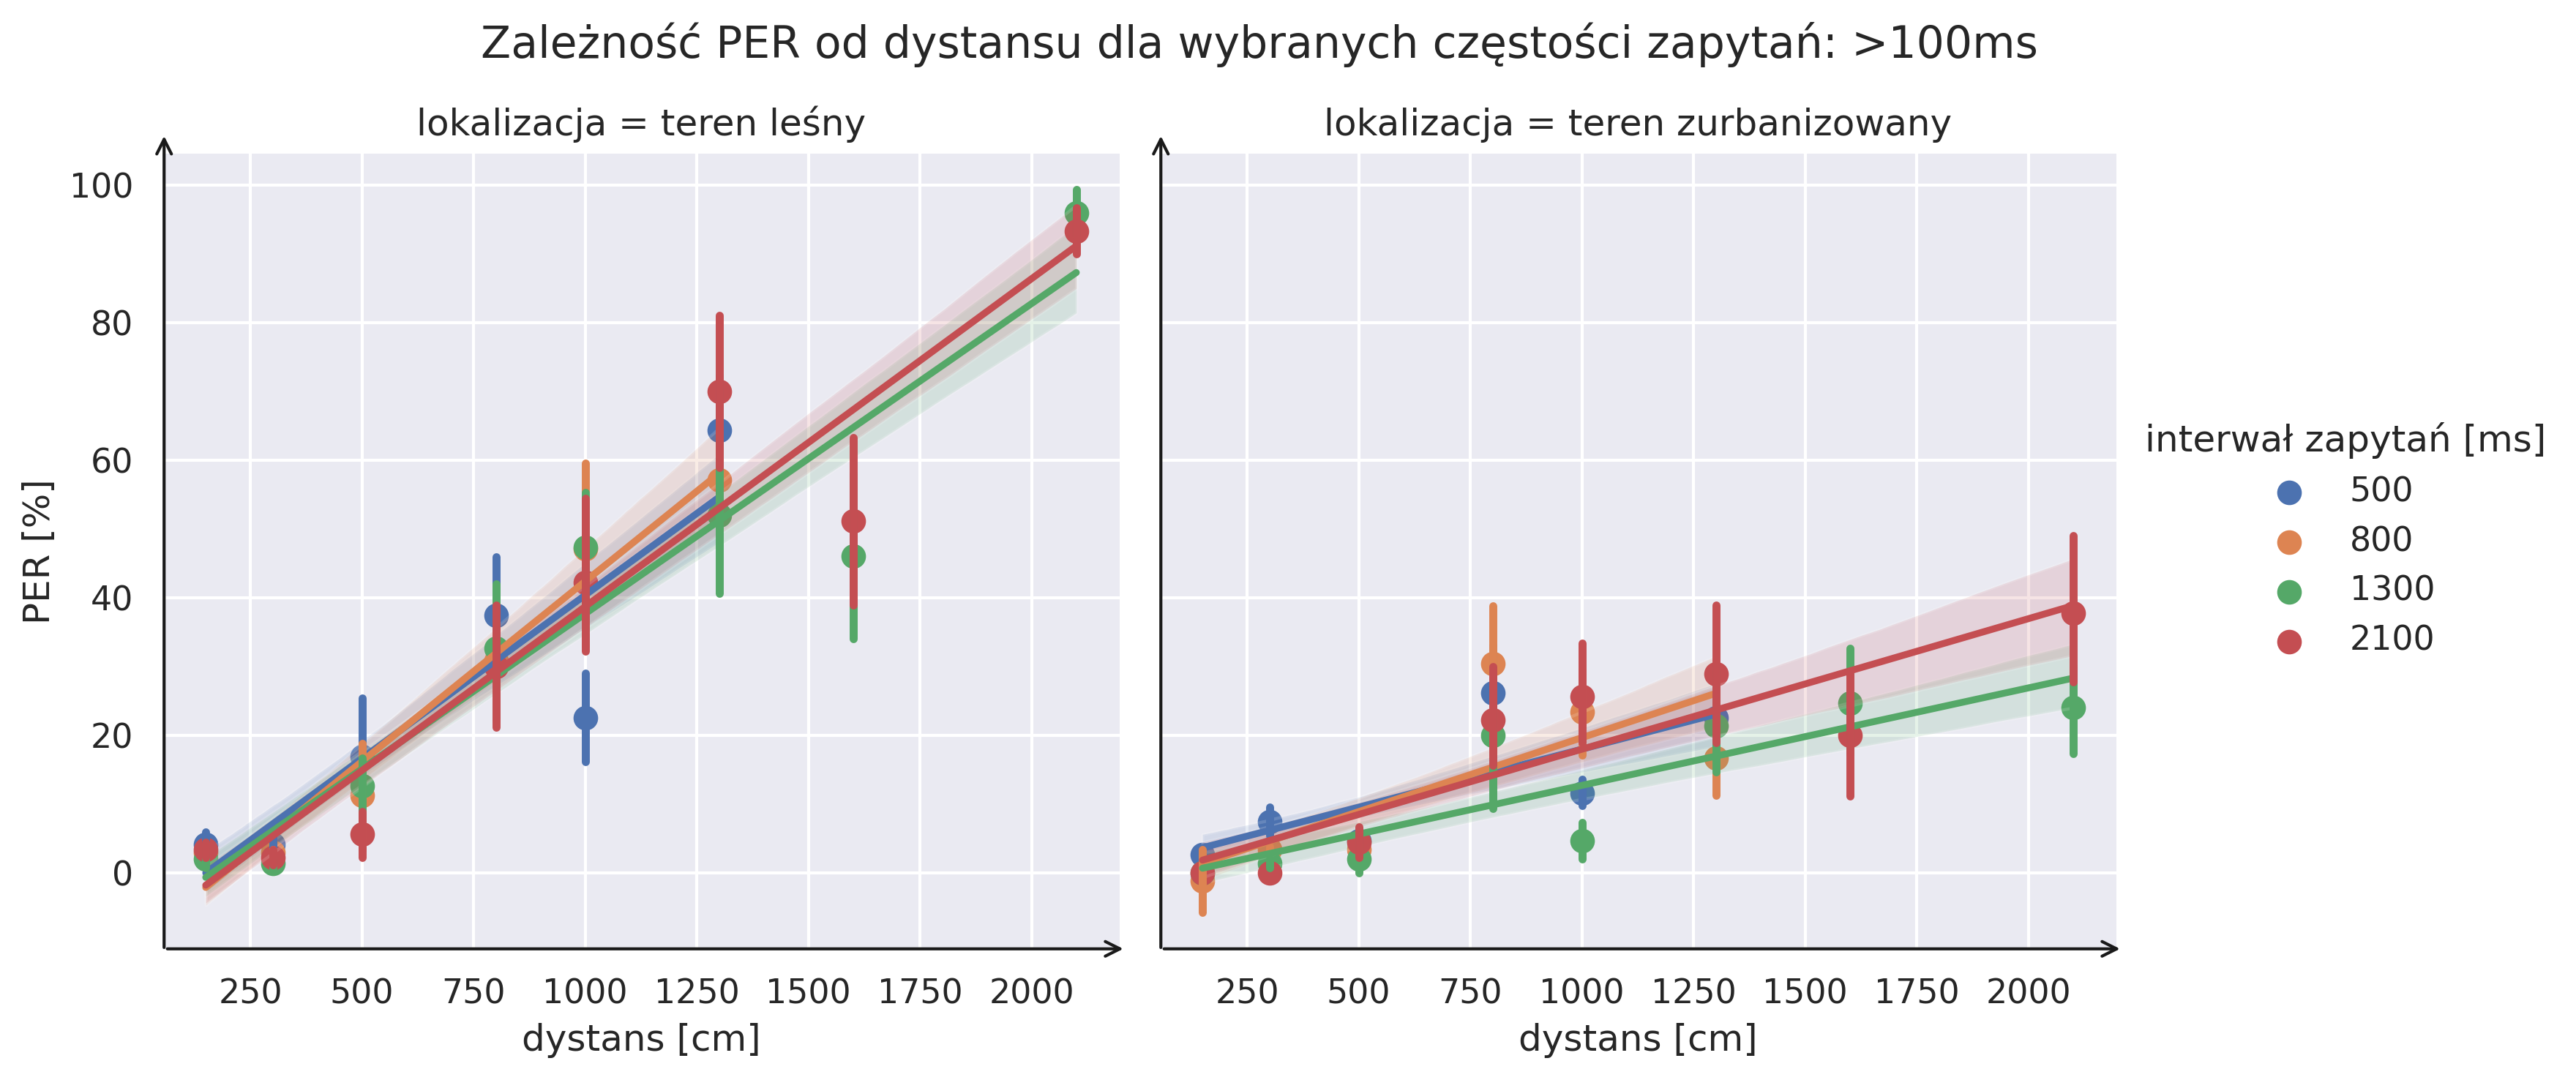
\includegraphics[width=0.99\linewidth]{per_to_distance_over_100ms_different_envs_different_ping_interval.png} 
	\caption{Zależność PER od dystansu dla zapytań o częstości >100ms w wybranych środowiskach}
	\label{rys:per_to_distance_over_100ms_different_envs_different_ping_interval}
\end{figure}


%%%%%%%%%%%%%%%%%%%%%%%%%%%%%%%%%%%%%%%%%%%%%%%%%%%%%%%%%%%%%%%%%%%%%%%%%%%%%%%%
%% SUBSECTION: Zależność PER względem odległości między węzłami
%%%%%%%%%%%%%%%%%%%%%%%%%%%%%%%%%%%%%%%%%%%%%%%%%%%%%%%%%%%%%%%%%%%%%%%%%%%%%%%%
\subsection{Zależność PER względem odległości między węzłami}

\begin{figure}[!htb]
	\centering 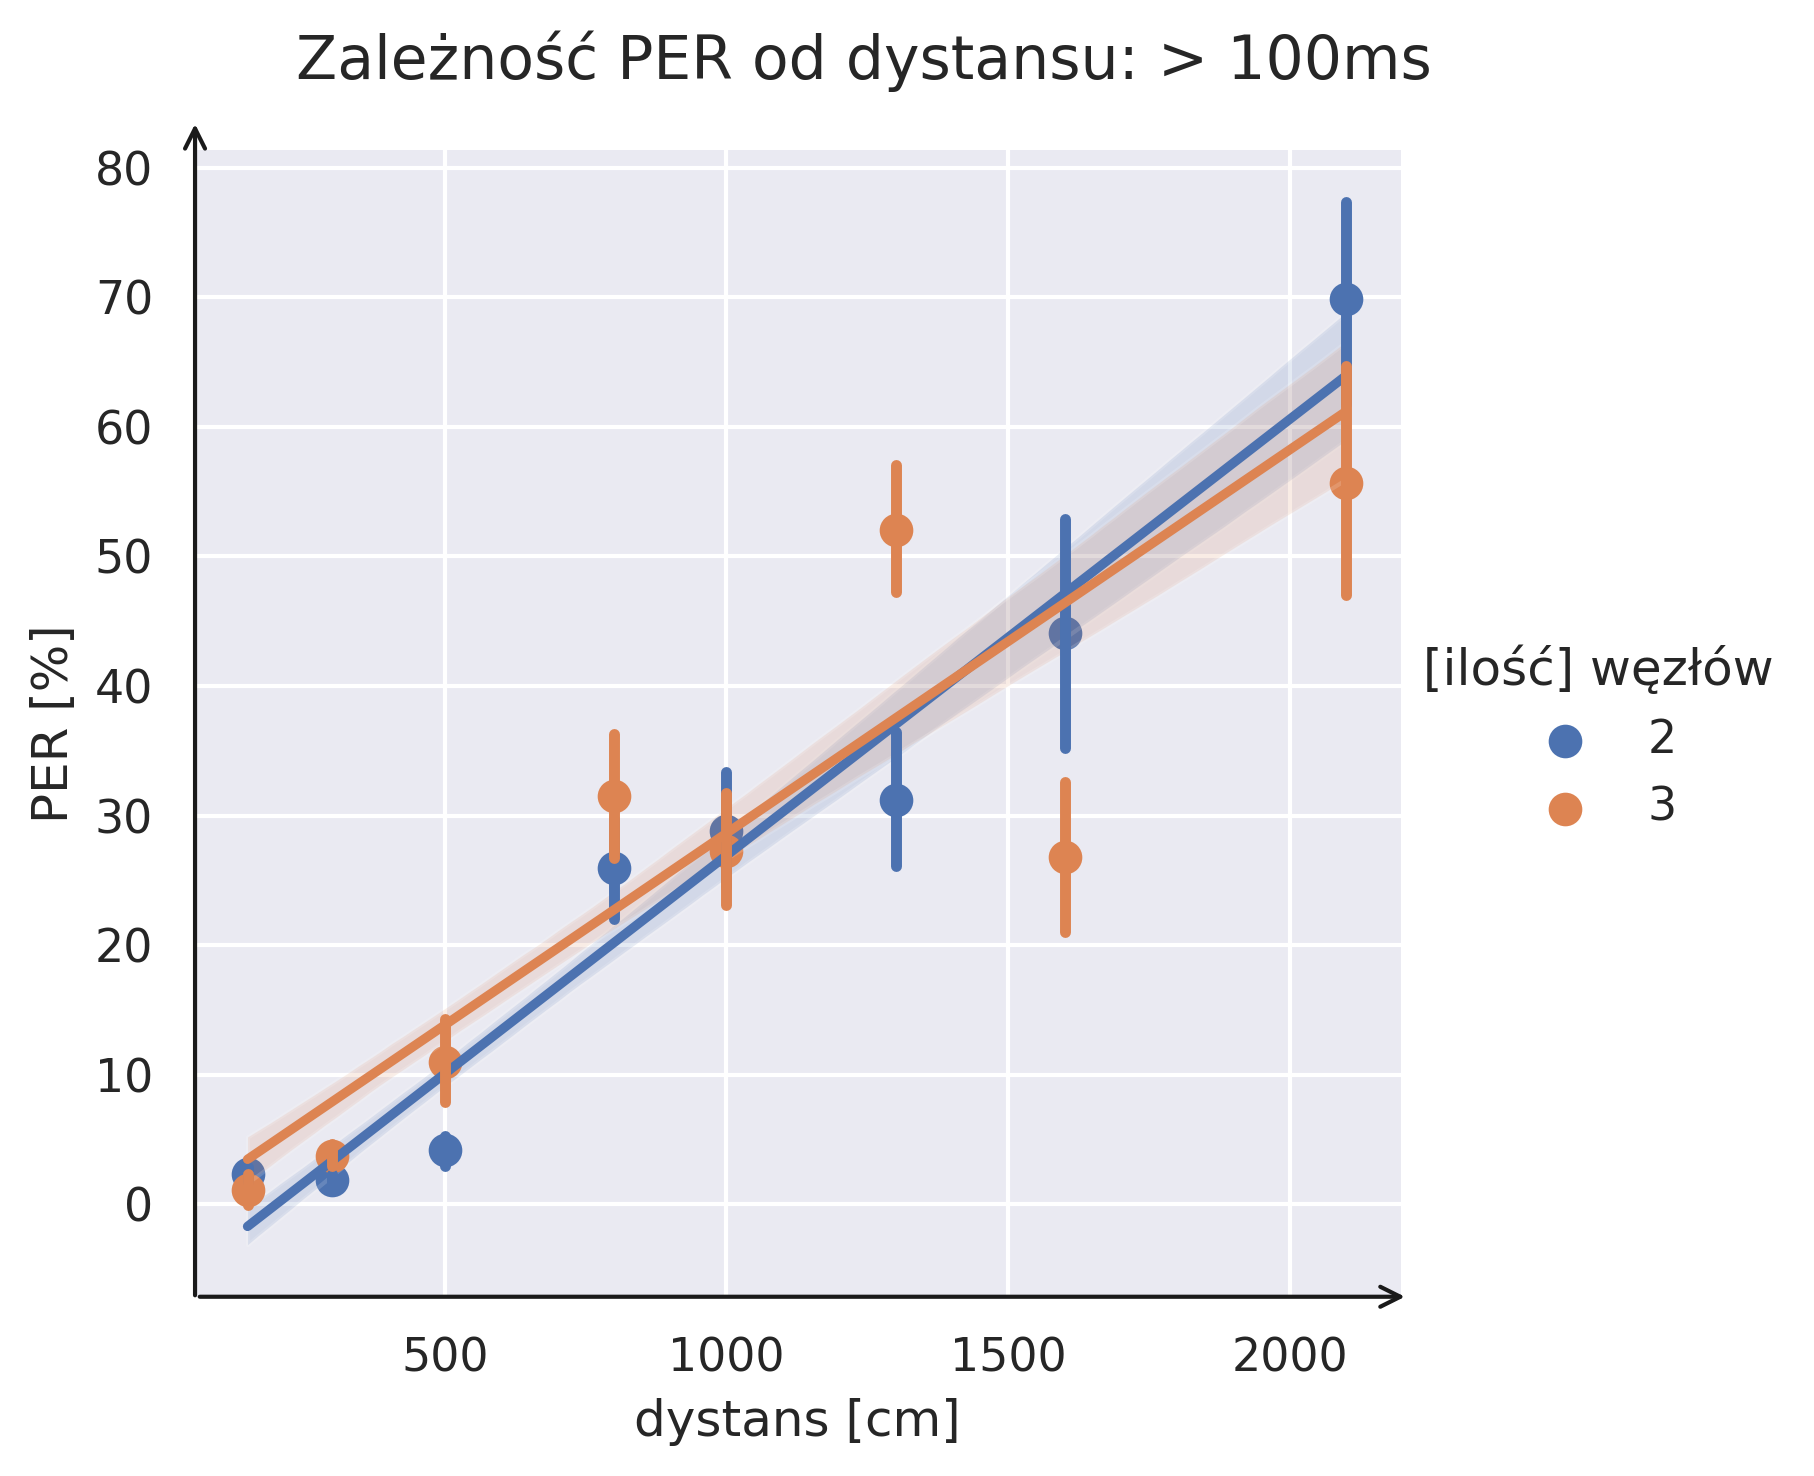
\includegraphics[width=0.618\linewidth]{per_to_distance_over_100ms.png}
	\caption{Zależność PER od dystansu dla zapytań o częstości >100ms dla różnej liczby węzłów}
	\label{rys:per_to_distance_over_100ms}
\end{figure}

\begin{figure}[!htb]
	\centering 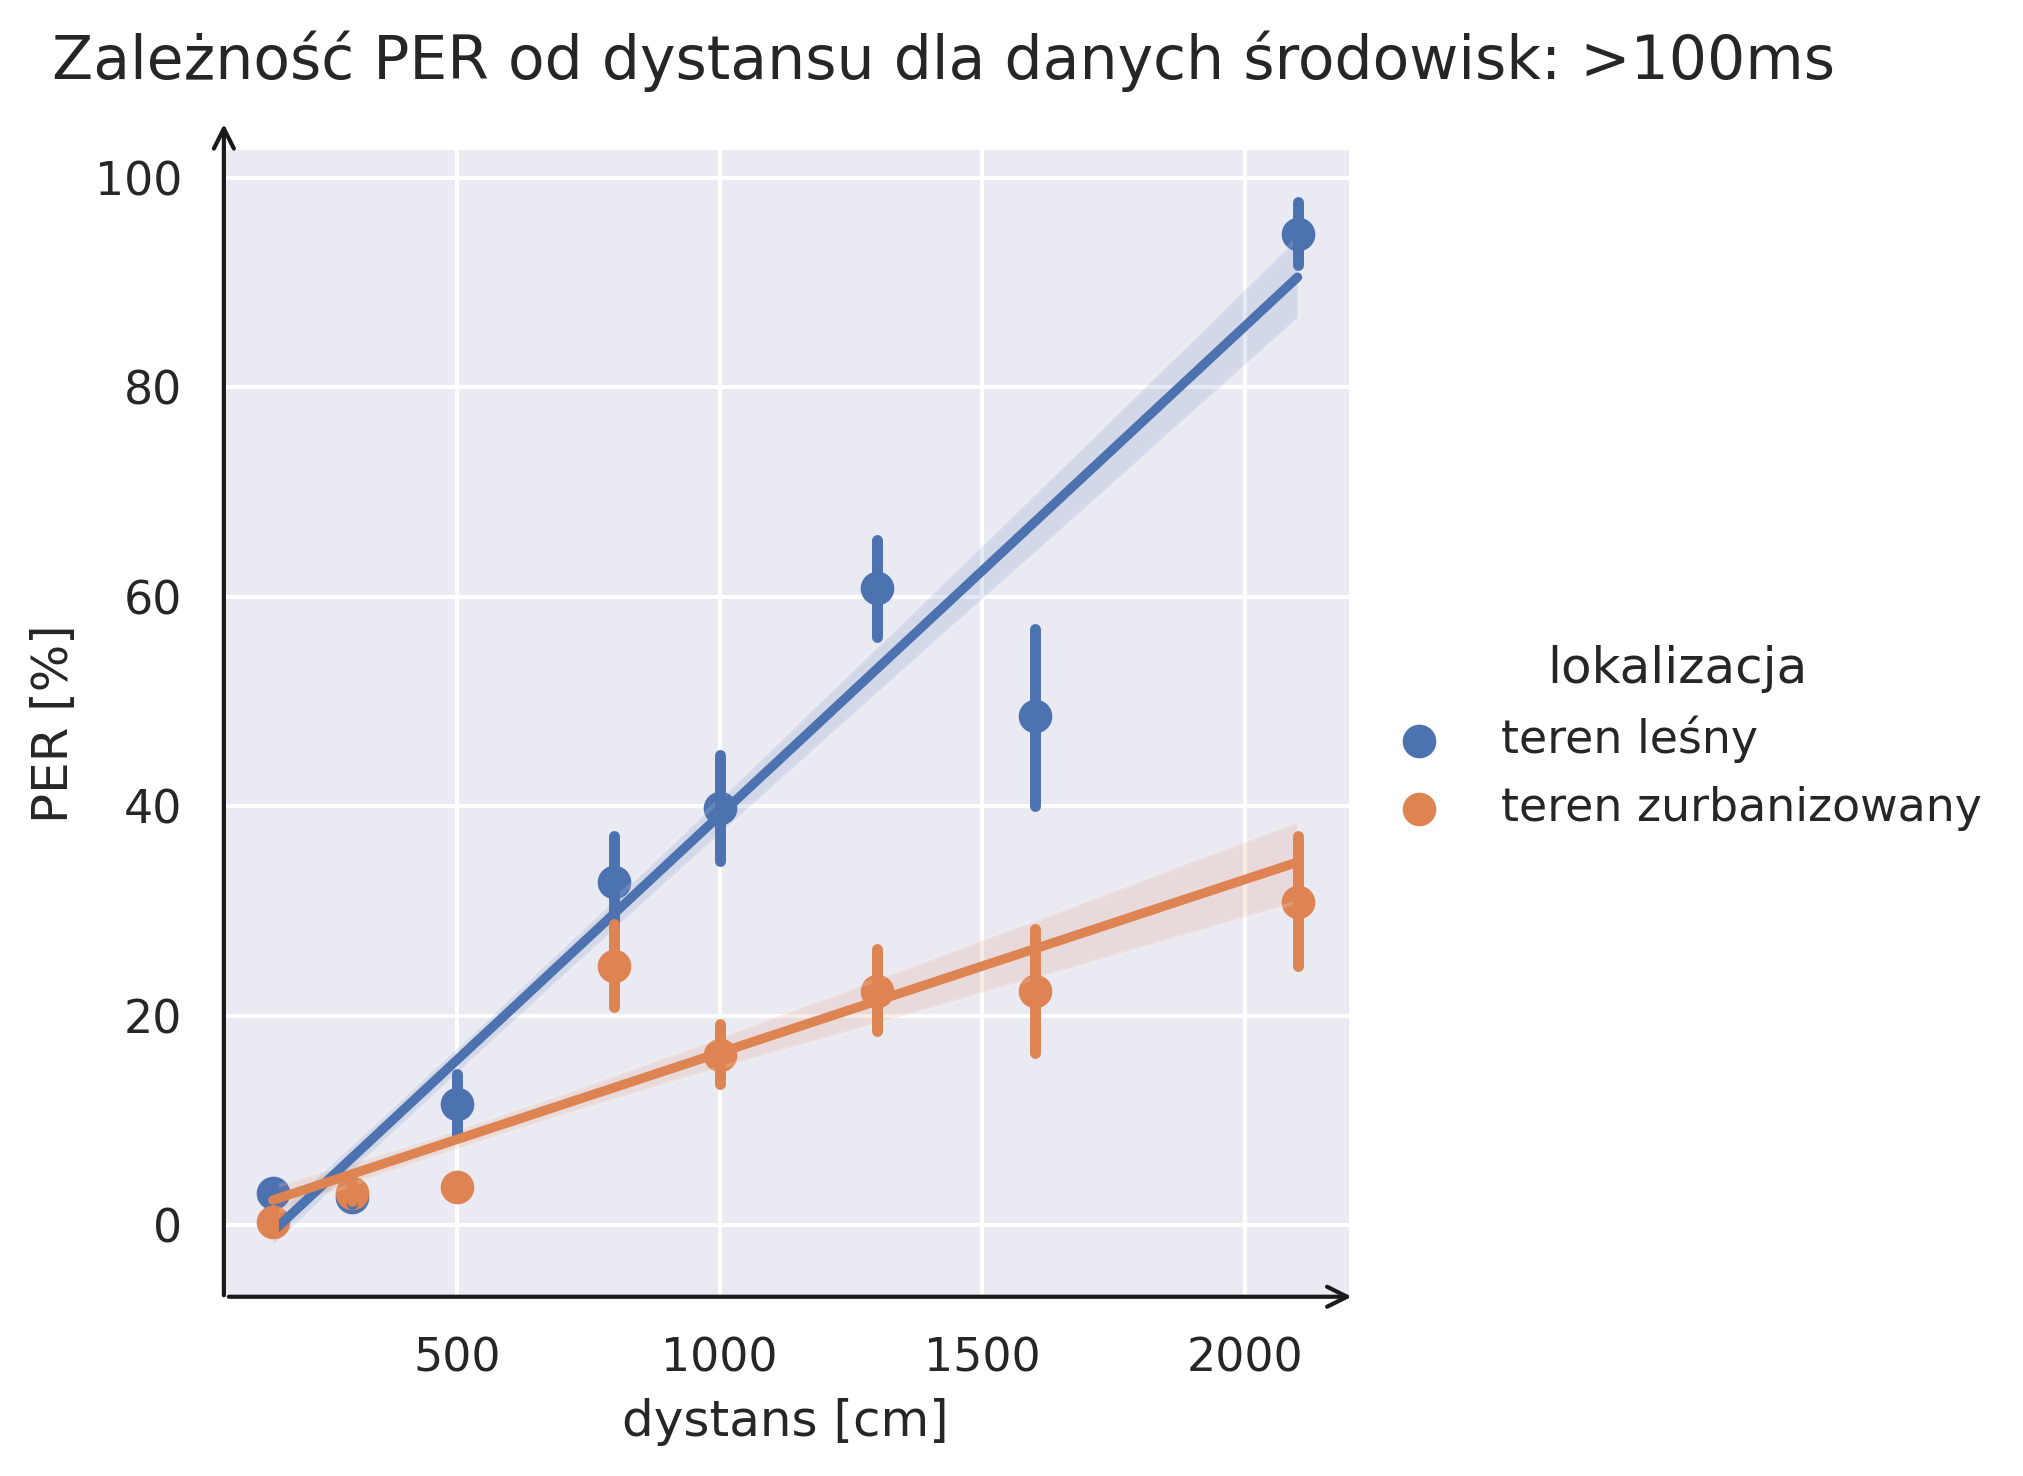
\includegraphics[width=0.618\linewidth]{per_to_distance_over_100ms_different_envs.png} 
	\caption{Zależność PER od dystansu dla zapytań o częstości >100ms w wybranych środowiskach bez rozróżnienia na liczbę węzłów}
	\label{rys:per_to_distance_over_100ms_different_envs}
\end{figure}

\begin{figure}[!htb]
	\centering 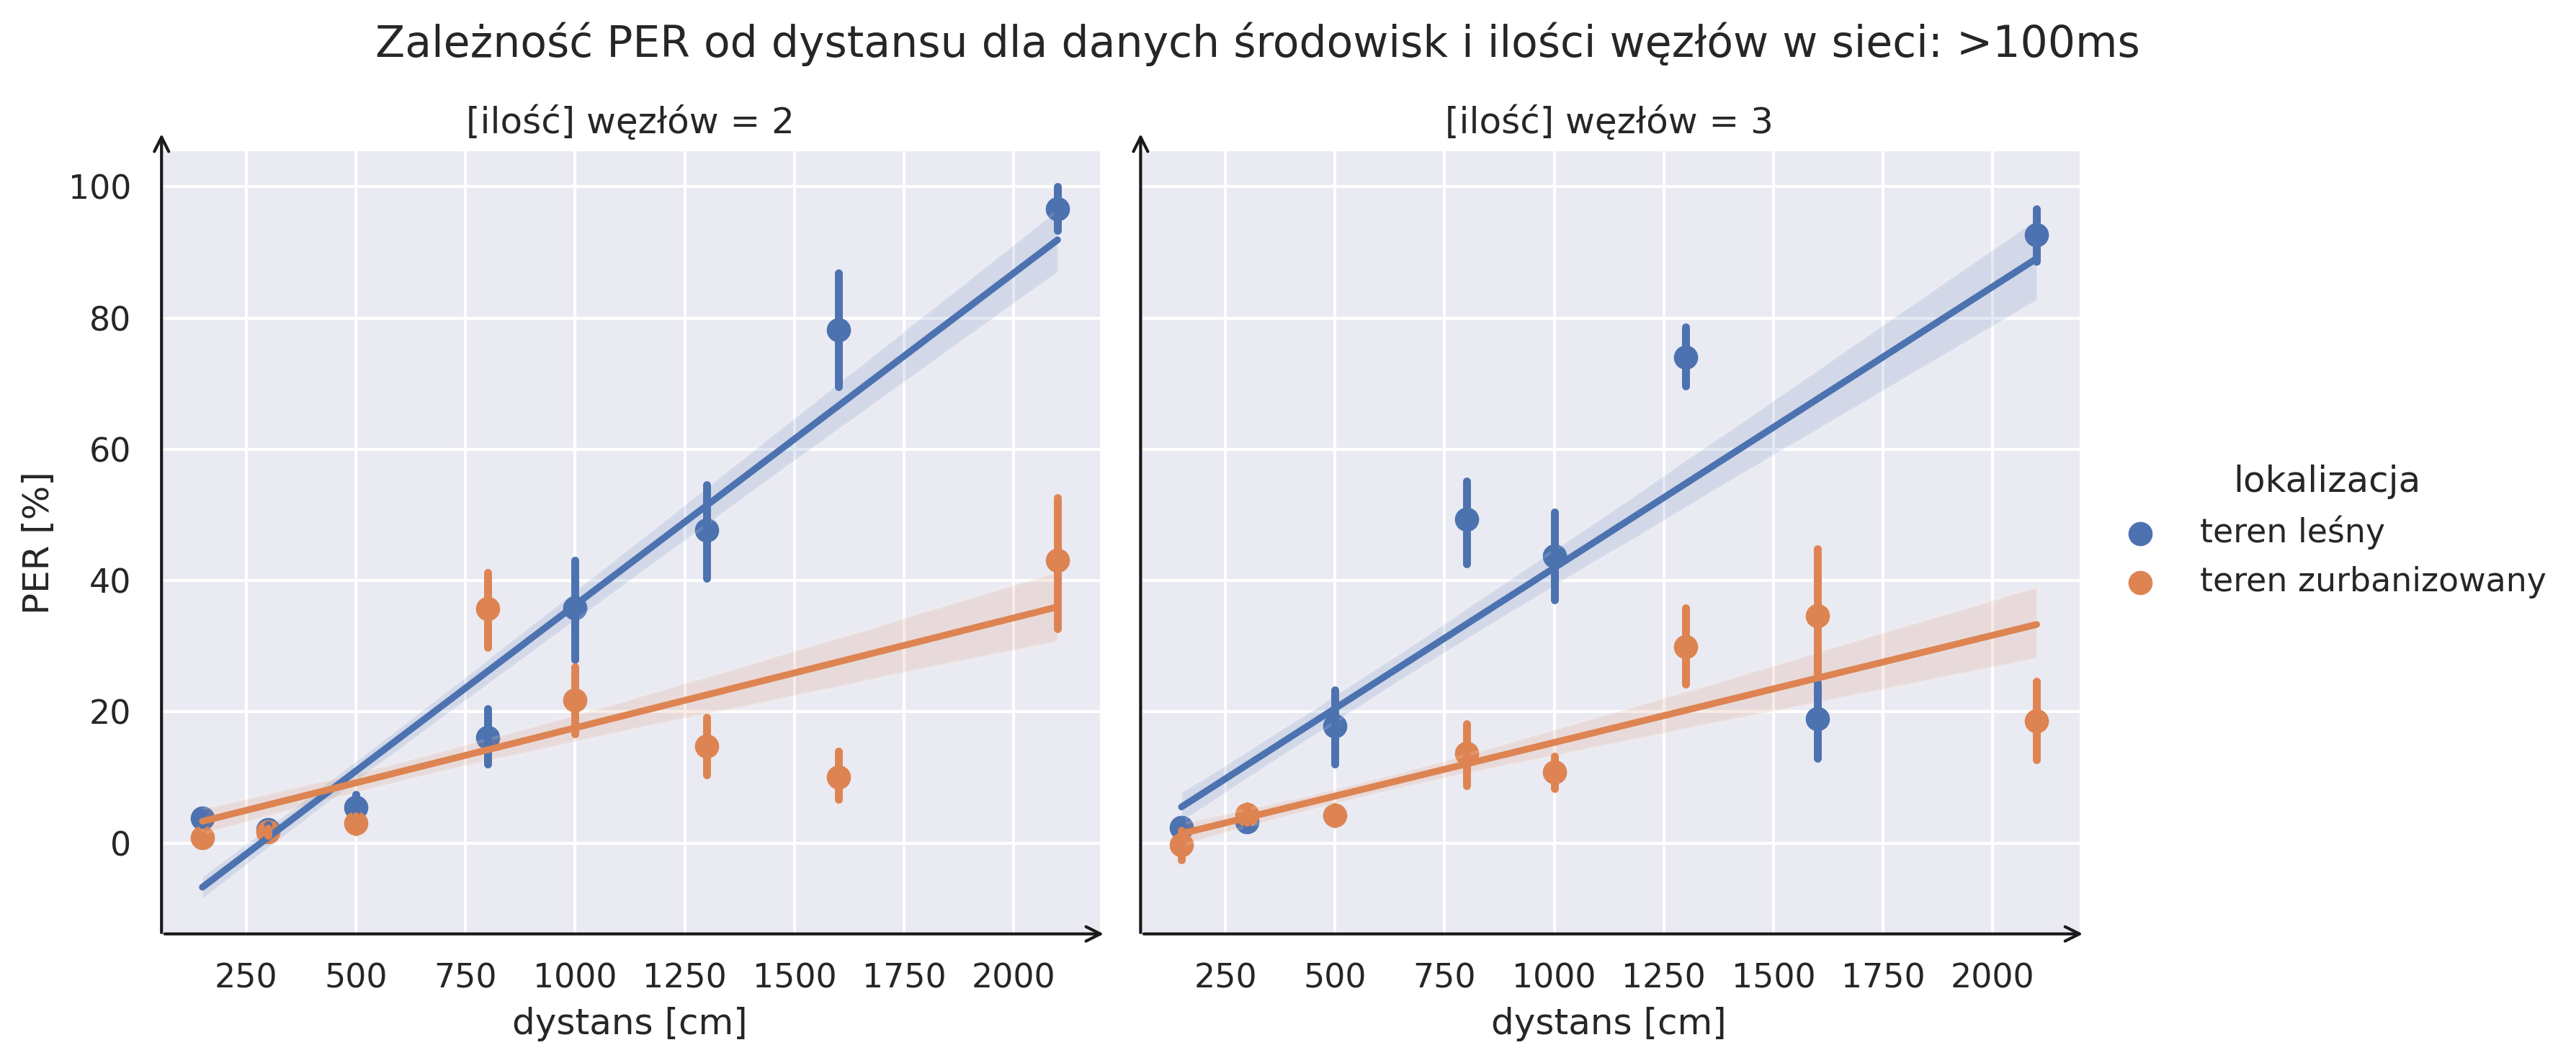
\includegraphics[width=0.99\linewidth]{per_to_distance_over_100ms_different_envs_and_nodes.png}
	\caption{Zależność PER od dystansu dla zapytań o częstości >100ms w wybranych środowiskach i liczbę badanych węzłów}
	\label{rys:per_to_distance_over_100ms_different_envs_and_nodes}
\end{figure}

